% =====================================================================
% 2026年度 修士論文（日本語版）
% OshiFit：個人の性格特性に適した推し活方法を提案するシステムの構築と検証
% コンパイル：upLaTeX → upBibTeX → upLaTeX ×2 → dvipdfmx
%   （Overleaf：Menu → Compiler を「LaTeX」にし、同梱の latexmkrc を使う）
% 体裁は2024年度卒業論文（表紙→概要→Abstract→目次→本文→参考文献→研究業績）に合わせた。
% 【要記入】【要確認】の箇所は、実験後・提出前に必ず埋める／確認すること。
% =====================================================================
\documentclass[uplatex,dvipdfmx,a4paper,11pt,openany]{jsreport}
\usepackage{graphicx}
\usepackage{amsmath,amssymb}
\usepackage{booktabs}
\usepackage{longtable}
\usepackage{array}
\usepackage{multirow}
\usepackage{url}
\usepackage[hidelinks]{hyperref}
\usepackage{pxjahyper}
\usepackage{caption}
\captionsetup{labelsep=colon}
\renewcommand{\thefigure}{\thechapter.\arabic{figure}}
\renewcommand{\thetable}{\thechapter.\arabic{table}}
\renewcommand{\bibname}{参考文献}

% 図表のキャプションを「図 1.1: 日本語 / Fig. 1.1: English」の2行にする（2024年度卒論の体裁）
\newcommand{\jecaption}[2]{\caption[#1]{#1\\{\small Fig.~\thefigure: #2}}}
\newcommand{\jetcaption}[2]{\caption[#1]{#1\\{\small Table~\thetable: #2}}}
% 実験後に埋める箇所
\newcommand{\todo}[1]{\textbf{【#1】}}
\newcommand{\placeholderfig}[2]{\fbox{\parbox[c][#1][c]{0.9\linewidth}{\centering\small #2}}}

% ---- 無料版Overleafでコンパイル時間が足りないとき ----
% 編集中の章だけをコンパイルする場合は，下の行の先頭の % を消して章のファイル名を指定する．
% （ページ番号・相互参照は前回の全体コンパイルの値が使われる．提出前は % を戻して全体をコンパイルする）
%\includeonly{chap3_survey}
% 図の読み込みを省いて速くする場合は，\documentclass の [ ] の中に draft を加える．
\begin{document}

% ---------------------------------------------------------------- 表紙
\begin{titlepage}
\begin{center}
{\Large 2026年度 修士論文}\\[34mm]
{\LARGE\bfseries OshiFit：個人の性格特性に適した\\[2mm]推し活方法を提案するシステムの構築と検証}\\[12mm]
{\large\bfseries OshiFit: Development and Evaluation of a System\\That Proposes Fan Activities (Oshi-katsu)\\Suited to Individual Personality Traits}\\[20mm]
{\large 指導教員}\\[2mm]
{\large 大井 翔 講師}\todo{要確認：職名}\\[14mm]
{\large M02530106\quad 今井 元}\\[6mm]
{\large 提出日：2027年1月}\\[30mm]
{大阪工業大学大学院 情報科学研究科\\メディアインタラクション研究室}\\[3mm]
{\small Media Interaction Laboratory, Graduate School of Information Science and Technology\\Osaka Institute of Technology}
\end{center}
\end{titlepage}

\pagenumbering{roman}
\chapter*{概要}
\addcontentsline{toc}{chapter}{概要}

本研究は，個人の性格特性と日々の推し活の状況から，その人に適した推し活方法を提案するシステム「OshiFit（オシフィット）」を構築し，その有用性を検証することを目的とする．

\paragraph{研究背景}
近年，精神的ストレスによるメンタル不調を抱える人は増加しており，精神疾患を有する総患者数は平成29年時点で約419.3万人に達している．ストレスを和らげる手段として，睡眠や運動に加えて趣味活動が注目されており，その中でも特定のアイドル，キャラクター，配信者などを継続的に応援する「推し活」は，Z世代を中心に広く行われている．推し活は「生きがい」や自己表現，人とのつながりをもたらす一方で，睡眠不足，過度な出費，「追わなければならない」という義務感，SNS上での他のファンとの比較による落ち込みといった負担（本研究では「推し疲れ」と呼ぶ）も生む．スクリーンタイムの制限や家計簿アプリは「減らすほど良い」ことを前提とするが，推し活では負担の原因となる活動が同時に生活の張りの源でもあるため，一律に減らす助言は楽しさまで奪う可能性がある．さらに，本人は自分のどの習慣が推し疲れにつながっているのかに気づきにくい．先行研究の多くは推し活の動機や心理を記述するにとどまり，便益と負担を同時に扱った定量的な検討や，個人の状態に合わせて推し活の仕方を支援する仕組みは十分に検討されていない．筆者の前研究（卒業論文）では，推し活時の心拍とストレスの関連を体験者3名・2週間で調べたが，体験者が少なく，受動的な推し活に限られ，期間も短いという課題が残った．

\paragraph{研究目的とリサーチクエスチョン}
本研究では，多くのファンの性格特性・推し活行動・幸福度・推し疲れの関係を分析し，その知見に基づいて，本人が自ら選べる提案と「今のまま続けた場合（プランA：現在のままの推し活）」と「提案を取り入れた場合（プランB：最適化された推し活）」の28日後の見込みを，自分に似せたアバターと数値で示すシステムを構築する．本人が気づきにくい負担の原因に気づき，自ら選んだ小さな変更によって幸福度の向上とストレスの軽減につなげることをねらう．次の3つのリサーチクエスチョン（RQ）を設定した．RQ1：性格特性（TIPI-J）と推し活行動は，幸福度・推し疲れとどのように関連し，個人の見込みをどの程度の精度で予測できるか．RQ2：約28日間の利用で，すでに良好な人（群A），プランBを選んだ人（群B），プランAを選んだ人（群C）の幸福度と推し疲れはそれぞれどう変化し，群の間でどう異なるか．RQ3：利用者は自分の推し疲れの原因に気づき，特に行動を変えた人はシステムを有用と評価するか．

\paragraph{調査（RQ1）}
推し活を行う日本のファンを対象にオンライン質問紙調査を行い，回答者234名から，推し活をしていない17名と注意確認項目に誤答した2名を除く215名（男性113名，女性94名，その他・無回答8名，年齢の中央値19歳）を分析した．性格特性はTIPI-Jの10項目（5件法），推し活行動は視聴・現地イベント・グッズ購入・SNSなどの頻度，推し活への没入，推し活をしたくなるきっかけ，推し活による幸福度と推し疲れを測定した．k-meansによる類型化，観測変数によるパスモデル，交互作用の検定，10分割交差検証による予測精度の推定を行った．その結果，79\%が推しを「生きがい」と答える一方で，40\%がお金の不安，33\%が睡眠への支障を報告し，幸福度と推し疲れは正の相関（$r=.24$）を示した．推し活の頻度は幸福度（$\beta=.43$）と推し疲れ（$\beta=.29$）の両方を高め，没入も両方に関連した（$\beta=.20$，$.23$）．すなわち，便益と負担は同じ行動から生じていた．性格特性は推し活の関わり方と関連した（外向性→頻度 $\beta=.19$，誠実性→没入 $\beta=-.15$，神経症傾向→気分の回復のための推し活 $\beta=.21$，開放性→同 $\beta=-.16$）が，頻度の効果を調整する効果は認められなかった（交互作用を加えても決定係数はほぼ変わらず，$p=.74$，$.79$）．性格のみによる類型化は分離が弱く（シルエット係数0.15〜0.18），性格は単独の「タイプ」としてではなく，行動と組み合わせて用いるのが適切であることが示された．性格・行動・きっかけを組み合わせた予測の交差検証決定係数は幸福度で.27，推し疲れで.11にとどまり，個人の予測には大きな不確かさが伴うことが分かった．

\paragraph{システム（OshiFit）}
これらの結果から，(D1)一律に減らす助言をせず「今のまま」も常に有効な選択肢とする，(D2)固定的な性格タイプではなく性格と本人の行動・負担を組み合わせて個人化する，(D3)便益と負担を同時に示す，(D4)予測の不確かさを正直に示す，という4つの設計指針を導いた．OshiFitは，質問紙（TIPI-J，推し活の内容の割合，気持ちと生活の変化，推し活をしたくなるとき，WHO-5，SHS，PSS-J．検証実験では短縮版の68問）から，幸福度・推し活の充実・睡眠と生活・お金・義務感と人間関係・SNSと比較の6軸を0〜100点で算出し，算出式と使用項目を画面に表示する．6軸のうち5軸以上が60点以上かつWHO-5の素点が13点以上の人には「今のままで順調」と伝え（群A），それ以外の人には，点数の低い軸に対応する15種類の提案から，性格の傾向と活動の比重も考慮して最大3案を示す．さらに，プランAとプランBの28日後の見込みを80\%の幅とともに示し，利用者が部品を選んで作った本人に似せたアバター（写真は使わない）の表情で，見込みの差を表す．利用者はプランBを選ぶ（群B）か，プランAを選ぶ（群C）かを自分で決め，約28日間，毎日のアンケート（約1分）と4日ごとの振り返り（全6回）で提案の実行状況と気分・推し疲れを記録する．見込みは本人の記録で少しずつ補正する．

\paragraph{検証実験（RQ2，RQ3）}
大阪工業大学の研究倫理審査の承認を得て，約28日間の検証実験を行う．群は無作為ではなく，開始時の状態（群A）と本人の選択（群B・C）で決まる．これは，趣味である推し活に変更を強制することが設計指針D1に反するためである．主要な結果指標はWHO-5と推し疲れ（総合）であり，各群の開始時と最後の調査の比較，開始時の値を共変量とした群Bと群Cの共分散分析，傾向スコアによる重み付けでの感度分析，毎日の記録の線形混合モデル，提案の実行の程度と変化量の関係（用量反応），見込みの当たり方を分析する．\todo{実験後に記入：参加者数，各群の人数，WHO-5と推し疲れの変化量と検定結果，気づき・有用性の評価結果}

\paragraph{本研究の意義}
本研究の意義は，第一に，推し活の便益と負担が同じ行動から生じることを215名の調査で定量的に示し，「減らせば良い」という支援が推し活には適さないことを明らかにした点にある．第二に，性格特性を固定的なタイプとしてではなく，行動・負担と組み合わせて個人化に用いるという設計の根拠を示した点にある．第三に，予測の不確かさを隠さずに示しながら，本人に似たアバターで2つの未来を比較させ，本人が自ら選ぶ行動変容を支援するシステムを構築した点にある．\todo{実験後に追記：検証実験から得られた知見}本研究の知見は，推し活に限らず，楽しさと負担が表裏一体となった趣味や娯楽を，やめさせるのではなく持続可能な形に整えるための支援の設計に応用できると考えられる．

\vspace{1em}
\noindent\textbf{キーワード：}推し活，ウェルビーイング，推し疲れ，性格特性（TIPI-J），パーソナルインフォマティクス，アバター，予測の不確かさ

\chapter*{Abstract}
\addcontentsline{toc}{chapter}{Abstract}

This study develops and evaluates OshiFit, a system that proposes ways of doing fan activities (\textit{oshi-katsu}) suited to each person, based on their personality traits and their current fan practices.

\paragraph{Background}
The number of people in Japan living with mental disorders has risen to about 4.19 million (2017), and hobbies are increasingly valued alongside sleep and exercise as a way of relieving stress. \textit{Oshi-katsu}, the sustained support of a favourite idol, character, or creator, is especially widespread among Generation Z. It gives fans a reason to live, a means of self-expression, and social connection, but it can also cause what fans call burnout: lost sleep, overspending, a sense of obligation to follow everything, and low mood from comparing themselves with other fans on social media. Screen-time limits and budgeting apps assume that less is better, yet in fan activities the practices that cause burden are often the same ones that make life meaningful, so blanket advice to cut down may remove the enjoyment as well. Moreover, fans rarely notice which of their own habits lead to burnout. Prior research has mostly described fans' motives and psychology; few studies have examined benefits and burdens together quantitatively, and none has supported individuals in adjusting how they engage. The author's previous study measured heart rate and stress during fan activities, but it involved only three participants over two weeks and covered mainly passive activities.

\paragraph{Aim and research questions}
This study analyses how personality traits, fan behaviours, well-being, and fan burnout relate across many fans, and builds a system that, based on these findings, offers proposals the user can choose and shows the predicted state after six weeks for keeping current habits (Plan A: current fan activities) and for adopting a proposal (Plan B: optimised fan activities), using a self-resembling avatar and scores with intervals. The aim is to help fans notice burdens they cannot easily see and to support self-chosen changes that raise well-being and reduce stress. Three research questions are addressed. RQ1: How are personality traits (TIPI-J) and fan behaviours associated with well-being and burnout, and how accurately can an individual's outlook be predicted? RQ2: Over six weeks of use, how do well-being and burnout change for fans who are already doing well (group A), who adopt Plan B (group B), and who keep Plan A (group C), within and between groups? RQ3: Do users recognise the sources of their burnout, and do those who changed their behaviour judge the system useful?

\paragraph{Survey (RQ1)}
An online survey of Japanese fans yielded 234 responses; after excluding 17 respondents with no fan activity and 2 who failed an attention check, 215 were analysed (113 men, 94 women, 8 other or undisclosed; median age 19). Personality (TIPI-J, 5-point), activity frequency, immersion, triggers for fan activity, well-being, and burnout were measured and analysed with k-means clustering, an observed-variable path model, moderation tests, and 10-fold cross-validated prediction. While 79\% said their \textit{oshi} gives them a reason to live, 40\% reported money worries and 33\% sleep disruption, and well-being and burnout were positively correlated ($r=.24$). Activity frequency was associated with both higher well-being ($\beta=.43$) and higher burnout ($\beta=.29$), as was immersion ($\beta=.20$, $.23$): benefits and burdens share the same sources. Personality was associated with how fans engage (extraversion with activity, $\beta=.19$; conscientiousness with lower immersion, $-.15$; neuroticism with mood-repair motives, $.21$; openness with weaker ones, $-.16$) but did not moderate the effect of activity ($p=.74$, $.79$). Clustering on personality alone separated poorly (silhouette 0.15--0.18). Cross-validated $R^2$ was .27 for well-being and .11 for burnout, showing that individual predictions are highly uncertain.

\paragraph{System}
Four design principles followed: (D1) never prescribe blanket reduction and always keep ``as is'' as a valid option; (D2) personalise by combining personality with the fan's own behaviours and burdens rather than assigning a fixed type; (D3) show benefits and burdens together; and (D4) be honest about uncertainty. From a 67-item questionnaire, OshiFit computes six axes on a 0--100 scale (well-being, enjoyment, sleep and daily life, money, obligation and relationships, social media and comparison) and shows each formula. Users with at least five axes $\geq 60$ and a WHO-5 raw score $\geq 13$ are told they are doing well (group A); others receive three of eleven proposals targeting their lowest axes, with ties broken by personality, and see Plan A and Plan B with 80\% intervals on a self-resembling avatar built on the device (the photo and landmarks are discarded). Users then choose Plan B (group B) or Plan A (group C) and complete weekly check-ins for six weeks.

\paragraph{Field study (RQ2, RQ3)}
After approval by the institutional ethics committee, a six-week field study is conducted. Groups are set by baseline state (A) and the user's own choice (B, C) rather than randomisation, because imposing changes on a hobby would contradict D1. The primary outcomes are WHO-5 and overall burnout, analysed within groups (baseline vs.\ week 6), across groups with A as reference (ANCOVA), between B and C with propensity-score weighting, and as a dose--response relationship within B. \textbf{[To be completed after the study: sample sizes, changes in WHO-5 and burnout, and ratings of awareness and usefulness.]}

\paragraph{Significance}
This study shows quantitatively that the benefits and burdens of fan activities arise from the same behaviours, so that ``do less'' support is unsuitable; provides evidence for using personality in combination with behaviour rather than as a fixed type; and builds a system that supports self-chosen behaviour change by comparing two futures on a self-resembling avatar while openly showing uncertainty. The approach may apply more broadly to hobbies and entertainment in which enjoyment and burden are intertwined, helping people sustain them rather than give them up.

\vspace{1em}
\noindent\textbf{Keywords:} oshi-katsu, fan activities, well-being, fan burnout, personality (TIPI-J), personal informatics, avatars, predictive uncertainty


\tableofcontents
\listoffigures
\listoftables
\clearpage
\pagenumbering{arabic}

\chapter{はじめに}
本章では，本研究の研究背景，先行研究の課題，研究目的とリサーチクエスチョン，本研究の貢献，および論文構成について述べる．

\section{研究背景}
\subsection{メンタル不調の増加とストレス対処}
近年，精神的ストレスによるメンタル不調を抱える人は増加している．厚生労働省の資料によると，精神疾患を有する総患者数は平成14年の約258.4万人から増加を続け，平成29年には約419.3万人（入院30.2万人，外来389.1万人）に達している\cite{mhlw2022}．McEwen\cite{mcewen1998}は，ストレスが心身に及ぼす影響を「アロスタシス」と「アロスタティック負荷」の概念で説明した．アロスタシスとは，環境的・心理的・社会的な変化に適応するために身体が生理的な仕組みを動員して安定を保とうとする働きであり，それが過剰に働き続けた結果として身体に蓄積される負担がアロスタティック負荷である．慢性的なストレスは心血管疾患や免疫機能の低下，精神疾患のリスクを高めるため，日常の中で適切にストレスを和らげる手段をもつことは心身の健康を保つうえで重要である．

ストレスを和らげる手段としては，睡眠や運動に加えて，趣味や娯楽の活動が重視されている．趣味は，日常の役割から離れて自分のための時間をもつこと，好きなものに没頭すること，同じものを好きな人とつながることを通じて，気分の回復や生活の張りをもたらす．一方で，趣味は「やめれば済む」ものではなく，本人にとっての生きがいと結びついているため，その付き合い方は本人が自ら選ぶものである点に特徴がある．

\subsection{推し活の広がり}
現在の日本では，特定のアイドル，アニメ・漫画・ゲームのキャラクター，VTuberや配信者，俳優，声優，スポーツ選手などを継続的に応援する「推し活」が広く行われている．推し活には，楽曲や動画の視聴，ライブやイベントへの現地参加，CD・Blu-rayやグッズの購入，テレビ・ラジオ・雑誌のチェック，SNSでの情報収集と発信，ロケ地を訪れる「聖地巡礼」，ファンクラブへの入会，コラボカフェへの来店，二次創作など，多様な形態がある．

株式会社ロイヤリティ マーケティングが2023年に10〜60代の推し活経験者879名に行った調査では，約半数（50.7\%）が推し活によって生活費に影響を感じていると回答し，20〜40代では約4割が月5,000円以上を推し活に使っていた\cite{loyalty2023}．Z世代を対象とした調査でも，6割以上が「推し」をもった経験があり，推し活の意義として「毎日を楽しくするもの」が最も多く挙げられている\cite{mery2023}．市場の面でも，矢野経済研究所の調査によれば，2024年度の「アイドル」市場は前年度比23.7\%増と大きく伸びており，ファンとの関係を軸にした体験型の消費が広がっている\cite{yano2026}．ファンの消費行動は，単なる購買ではなく自己のアイデンティティを映す「鏡」としての意味をもつことも指摘されている\cite{sandvoss2005}．

\subsection{推し活の便益と負担}
推し活は，ファンに多くの便益をもたらす．推しの存在が毎日の活力となり，つらいときに気持ちを支え，同じ推しを応援する仲間とのつながりを生む．井上・上田\cite{inoue2023}は，アイドルに対するファンの心理的所有感（「自分たちの推し」という感覚）が幸福感と関連することを示し，上田・井上\cite{ueda2023}は，推し活意識が推しへの心理的所有感を介して幸福感を高めることを報告している．宮田\cite{miyata2024}も，推し活が幸福度にもたらす意味を考察している．女子大学生を対象とした市村\cite{ichimura2025}の調査は，推し活が「ファン活動」「オタク活動」とは異なる肯定的なイメージで捉えられていることを示した．

一方で，推し活は負担も生む．夜遅くまで配信を見たりSNSを追ったりすることによる睡眠不足，予算を超えたグッズの購入やくじへの出費，「すべてのイベントに参加しなければならない」「情報を追い続けなければならない」という義務感，SNS上で他のファン（同担）の活動を見て嫉妬したり落ち込んだりすること，ファン同士の人間関係の疲れなどである．本研究では，これらをまとめて「推し疲れ」と呼ぶ．推し疲れは，対人援助職などで研究されてきたバーンアウト（燃え尽き）\cite{maslach1981,kubo2007}と同様に，熱心に関わるほど生じやすいという特徴をもつと考えられる．

重要なのは，推し活では便益をもたらす活動と負担をもたらす活動が同じであることが多い点である．スクリーンタイムを制限するアプリや家計簿アプリは「減らすほど良い」ことを前提としているが，推し活において一律に活動を減らす助言をすると，負担だけでなく楽しさや生きがいまで失わせてしまう可能性がある．また，本人は自分のどの習慣が推し疲れにつながっているのかに気づきにくい．推し活を続けたまま負担を減らすには，その人の状態に合わせて「何をどう変えるか」を本人が選べる形で示す支援が必要である．

\subsection{筆者の前研究}
筆者は卒業研究\cite{imai2025thesis,imai2025hr}において，推し活時の心拍とストレスの関連を調べた．質問紙の回答から推し活のタイプを13種類に分類し，タイプの異なる体験者3名にスマートウォッチ（Garmin Vivosmart 4）を2週間装着してもらい，推し活前と推し活中の心拍数を比較した．その結果，1名では推し活前と推し活中の平均心拍数に有意差が認められたが，他の2名では認められなかった．また，主な推し活が動画視聴であったことから，受動的な推し活が副交感神経を優位にしてリラックスをもたらす可能性が考えられた一方，高ストレス状況下では推し活の肯定的な効果が抑えられる傾向も自由記述からうかがえた．

この前研究には，(1)体験者が3名と少なく統計的な一般化が難しいこと，(2)対象がライブやイベントのような能動的な推し活を含まない受動的な推し活に偏っていたこと，(3)期間が2週間と短く，継続的な効果を検証できなかったこと，(4)推し活の状態を測ることにとどまり，本人の推し活をより良くするための支援にはつながっていないこと，という課題が残った．本研究はこれらの課題を受け，多数のファンを対象とした調査と，個人に合わせた提案を行うシステムの構築・検証へと発展させるものである．

\section{先行研究の課題}
推し活やファン行動に関する先行研究（第2章で詳述）は，主に次の3点で課題を残している．

\begin{enumerate}
\item \textbf{便益と負担を同時に扱った定量的な検討が少ない．}多くの研究は推し活の動機や心理的な便益を扱うか，負担を個別に扱うにとどまり，同じ人の中で便益と負担がどのような行動から生じるのかを同時に分析した研究は少ない．
\item \textbf{個人差の扱いが記述にとどまる．}性格特性や心理的傾向とファン行動の関連は報告されているが，それを個人に合わせた支援にどう生かすか（性格を固定的な「タイプ」として扱うのか，行動と組み合わせて扱うのか）は実証的に検討されていない．
\item \textbf{個人を支援する仕組みがない．}パーソナルインフォマティクスの分野では，記録を見せるだけでは行動が変わりにくいことが知られている\cite{li2010,choe2014}．推し活においても，本人が自分の状態に気づき，自ら選んだ変更を試せるような支援の仕組みは検討されていない．
\end{enumerate}

\section{研究目的とリサーチクエスチョン}
本研究の目的は，多くのファンの性格特性・推し活行動・幸福度・推し疲れの関係を分析し，その知見に基づいて，本人が自ら選べる提案と「今のまま続けた場合」と「提案を取り入れた場合」の見込みを示すシステムOshiFitを構築し，その有用性を検証することである．OshiFitは，本人に似たアバターを用いて，プランA「現在のままの推し活」とプランB「最適化された推し活」の6週間後の幸福度と推し疲れの見込み（本研究ではこの差を「ウェルビーイング・ギャップ」と呼ぶ）を示す．これにより，本人が気づきにくい負担の原因に気づき，自ら選んだ小さな変更によって幸福度の向上とストレスの軽減につなげることをねらう．図\ref{fig:flow}に，OshiFitの5つの段階と本研究の各部分の対応を示す．

\begin{figure}[t]
\centering
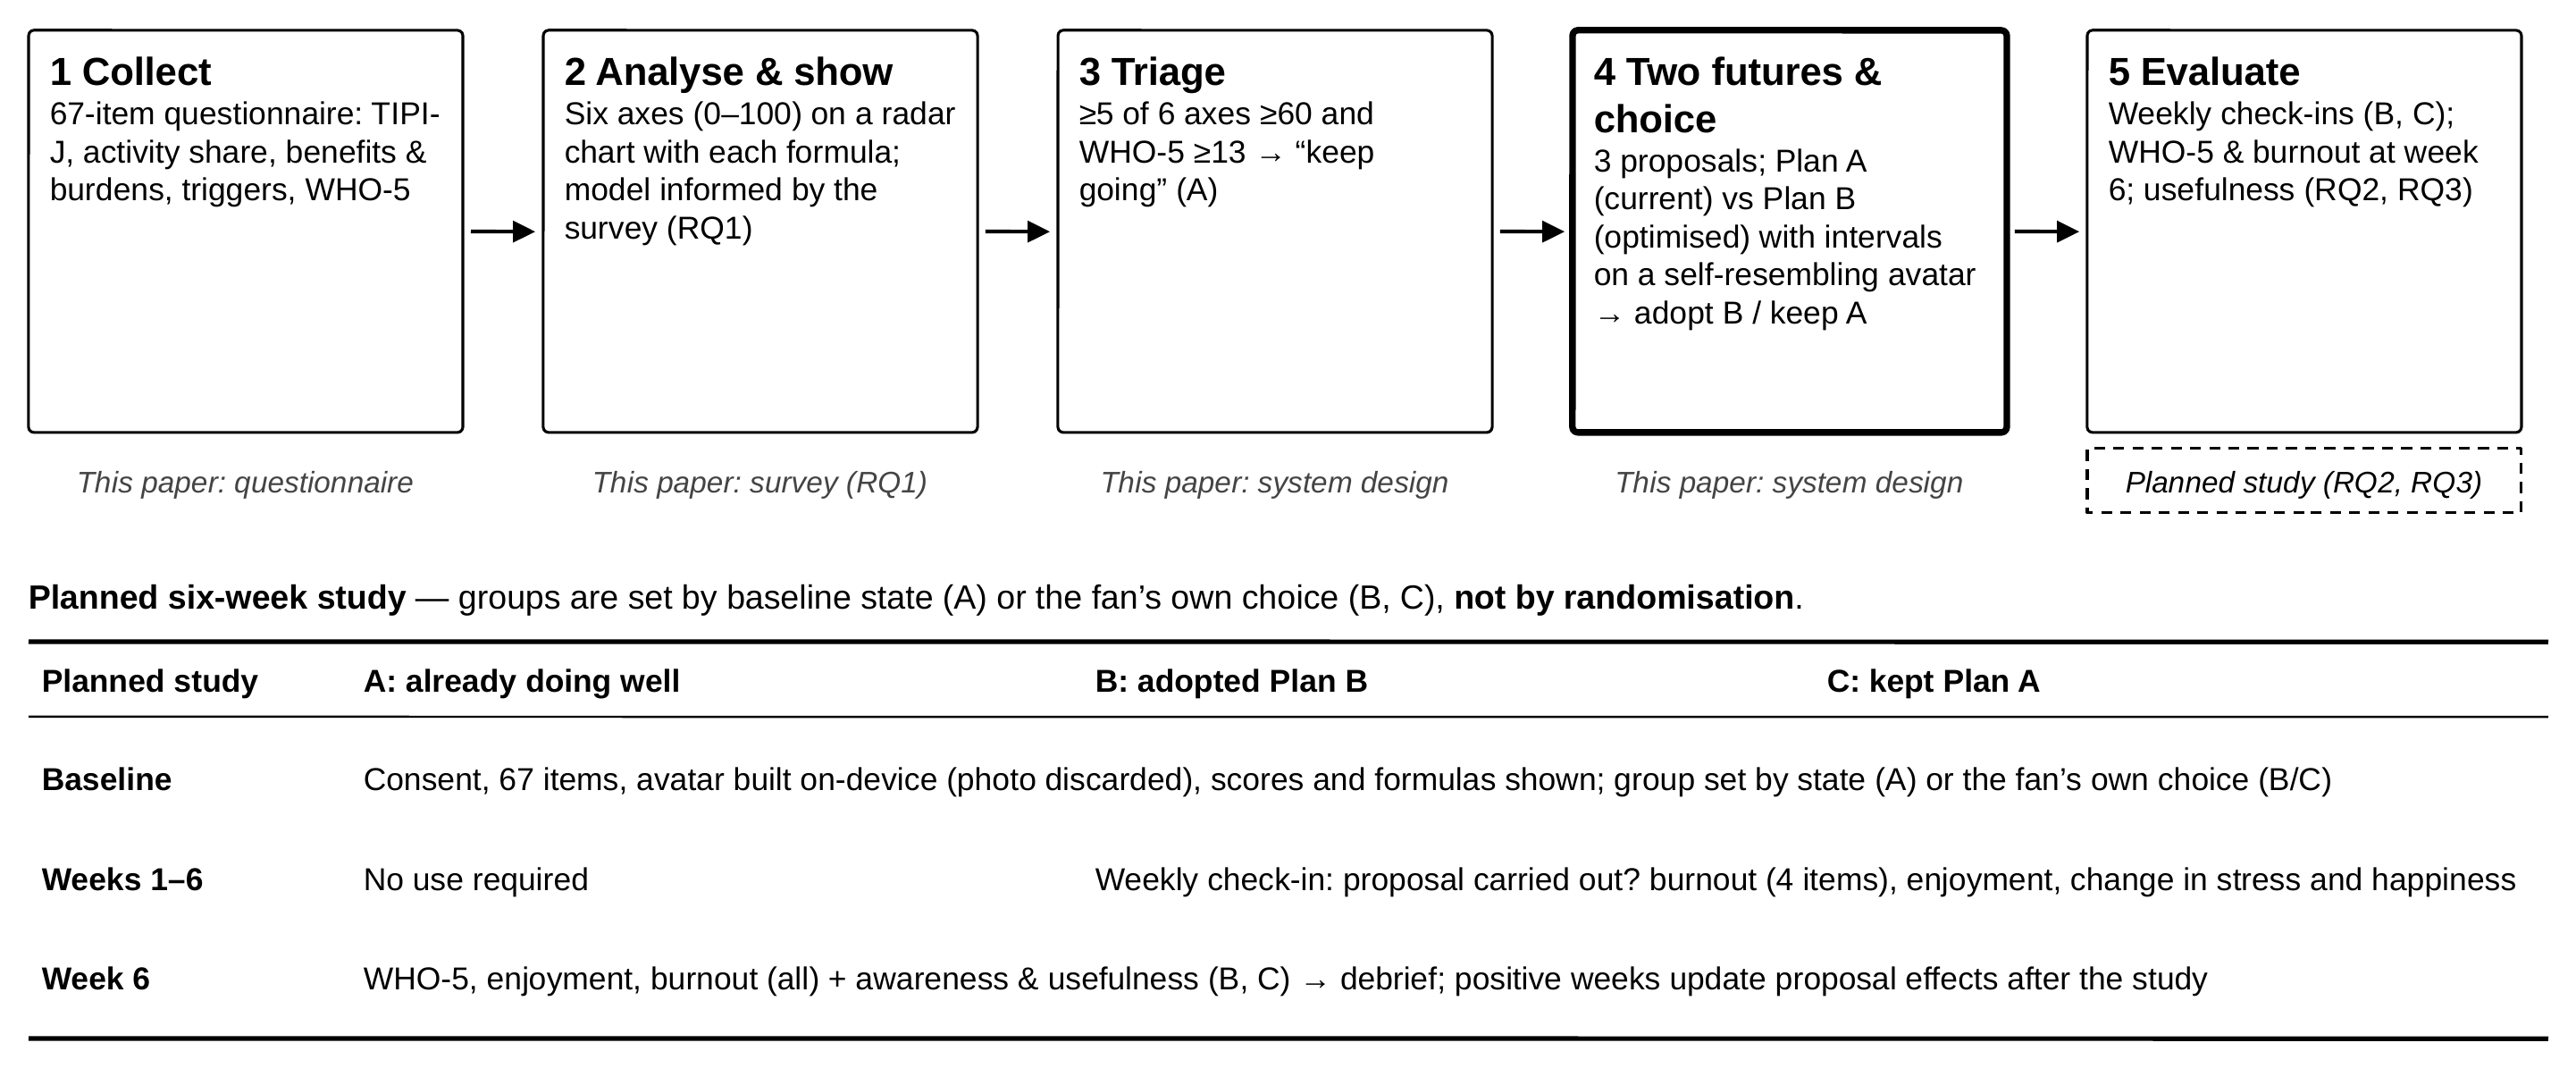
\includegraphics[width=\linewidth]{figures/fig1_flow_ppt.png}
\jecaption{OshiFitの5つの段階（上）と6週間の検証実験の計画（下）}{Five stages of OshiFit (top) and the planned six-week study (bottom)}
\label{fig:flow}
\end{figure}

本研究では，次の3つのリサーチクエスチョンを設定する．

\begin{description}
\item[RQ1] 性格特性（TIPI-J）と推し活行動は，幸福度・推し疲れとどのように関連し，個人の見込みとしてどの程度の精度で予測できるか．
\item[RQ2] 6週間の利用で，すでに良好な人（群A），プランBを選んだ人（群B），プランAを選んだ人（群C）の幸福度と推し疲れは，それぞれの群の中でどう変化し，群の間でどう異なるか．
\item[RQ3] 利用者は自分の推し疲れの原因に気づき，特に行動を変えた人はシステムを有用と評価するか．
\end{description}

RQ1には215名の質問紙調査で答え（第3章），その結果からシステムの設計指針を導いてOshiFitを構築する（第4章）．RQ2とRQ3には6週間の検証実験で答える（第5章）．

\section{本研究の貢献}
本研究の貢献は次の4点である．
\begin{enumerate}
\item 215名の調査により，推し活の便益（幸福度）と負担（推し疲れ）が同じ行動から生じることを定量的に示し，推し活の支援は「減らす」ことではなく「整える」ことを目指すべきであるという根拠を示した．
\item 性格特性は推し活の関わり方と関連するが，行動の効果を調整するわけではないことを示し，性格を固定的なタイプとしてではなく行動と組み合わせて個人化に用いるという設計の根拠を示した．
\item 個人の予測には大きな不確かさが伴うことを示し，予測を幅とともに正直に示す設計を導いた．
\item これらの知見を4つの設計指針にまとめ，本人に似たアバターで2つの未来を比較し，自ら選んだ行動変容を支援するシステムOshiFitを構築し，6週間の検証実験でその有用性を検討した．
\end{enumerate}

\section{論文構成}
本論文は全7章で構成される．第2章では，推し活・ファン行動，ウェルビーイングと負担，性格特性と個人化，パーソナルインフォマティクスと行動変容，アバターと将来の自己，予測の不確かさの提示に関する関連研究を概観し，本研究の位置付けを述べる．第3章では，RQ1に答えるための質問紙調査の方法と結果を述べ，システムの設計指針を導く．第4章では，OshiFitの設計と実装について述べる．第5章では，RQ2とRQ3に答えるための6週間の検証実験の方法と結果を述べる．第6章では，得られた知見を総合的に考察し，本研究の限界を述べる．第7章では，本研究をまとめ，今後の展望を述べる．

\chapter{関連研究}
本章では，本研究に関連する先行研究として，推し活・ファン行動に関する研究，推し活とウェルビーイング・負担に関する研究，性格特性と個人化に関する研究，パーソナルインフォマティクスと行動変容に関する研究，アバターと将来の自己に関する研究，予測の不確かさの提示と推薦の説明に関する研究，生理指標によるストレス計測に関する研究を概観し，本研究の位置付けを述べる．

\section{推し活・ファン行動に関する研究}
ファン行動は，社会学やメディア研究の分野で古くから扱われてきた．Sandvoss\cite{sandvoss2005}は，ファンが対象に向ける熱中を，消費を通じて自己を映し出す「鏡」として捉え，ファンであることが個人のアイデンティティと深く結びついていることを論じた．

日本のファン心理については，吉田\cite{yoshida2010}が自己愛傾向とファン行動の関連を調べ，ファン行動の質問項目に基づくクラスタリングにより，自己愛傾向がファン行動のあり方に関わることを示した．小城\cite{koshiro2018}は，ファン心理尺度を再検討し，ファンが対象に向ける心理を多面的に測定する尺度を提案している．これらの研究は，ファン行動に個人差があり，その背景に心理的な傾向があることを示しているが，個人を支援することは目的としていない．

近年は「推し」や「推し活」という言葉そのものを対象とした研究も増えている．市村\cite{ichimura2025}は，女子大学生を対象に「ファン活動」「オタク活動」「推し活」のイメージと推し活を行う理由を調べ，推し活が肯定的なイメージをもつ活動として捉えられていることを示した．本間ら\cite{homma2025}は，「推し」がどのように形成され，何がそれを決めるのかをモデル化することを試みている．東ら\cite{higashi2024}は，「推し」を認知科学の観点から捉える応援研究の進展と可能性を論じている．これらの研究は推し活という現象の理解を深めているが，推し活の負担や，その個人に合わせた支援までは扱っていない．

\section{推し活とウェルビーイング・負担に関する研究}
推し活が幸福感にもたらす効果については，いくつかの定量的な検討がある．井上・上田\cite{inoue2023}は，アイドルに対するファンの心理的所有感が幸福感と関連すること，また他のファンへの意識（競争的な意識）が応援の継続を妨げうることを示した．上田・井上\cite{ueda2023}は，推し活意識が推しへの心理的所有感を媒介して幸福感を高めることを報告している．宮田\cite{miyata2024}は，幸福度と推し活の関係について考察している．

幸福やウェルビーイングの捉え方としては，人生への満足や主観的な幸福感を中心とする立場と，人生の意味や成長，他者とのよい関係などを含む心理的ウェルビーイングを重視する立場がある．西田\cite{nishida2000}は，成人女性を対象に心理的well-beingを多面的に測定する尺度を作成している．大野\cite{ono1984}は，青年の「充実感」を測定する尺度を作成し，生活への張りや主体性といった側面を捉えている．主観的幸福感については日本版主観的幸福感尺度（SHS）\cite{shimai2004}が，精神的健康の簡便な指標としてはWHO-5\cite{topp2015}とその日本語版\cite{inagaki2013}が広く用いられている．自己決定理論\cite{ryan2000}は，自律性・有能感・関係性の欲求が満たされることがウェルビーイングを支えるとしており，推し活において本人が自分で選ぶことや仲間とのつながりが重要であることとも整合する．

一方，熱心な関わりが疲弊を生むことは，対人援助職などのバーンアウト研究で知られている．Maslach と Jackson\cite{maslach1981}は，情緒的消耗感などからなるバーンアウトの測定尺度を提案し，久保\cite{kubo2007}は日本のヒューマンサービス職におけるバーンアウトを整理している．推し活における負担は職業上のバーンアウトとは異なるが，対象への強い関与が疲れを生むという点で共通する．しかし，推し活の便益と負担を同じ人の中で同時に測定し，それらがどの行動から生じるのかを分析した研究はほとんどない．

\section{性格特性と個人化に関する研究}
性格特性の代表的な枠組みとして，外向性・協調性・誠実性・神経症傾向・開放性の5因子からなるビッグファイブがある．Goslingら\cite{gosling2003}は，各因子を2項目，計10項目で測定する短縮版尺度TIPIを開発し，小塩ら\cite{oshio2012}はその日本語版TIPI-Jを作成して信頼性と妥当性を検討した．TIPI-Jは回答の負担が小さいため，アプリの中で利用者の性格を把握する用途に適している．

推薦システムや健康支援の分野では，利用者の性格に合わせて推薦や介入を個人化する試みがある．しかし，性格をどのように個人化に用いるべきか，すなわち性格を固定的な「タイプ」として扱い，タイプごとに決まった推薦を行うのか，それとも性格が行動や関わり方とどう結びついているかを踏まえて行動と組み合わせて用いるのかは，対象領域ごとに実証的に確かめる必要がある．推し活においてこの点を検討した研究はない．

\section{パーソナルインフォマティクスと行動変容に関する研究}
自分に関するデータを収集し，振り返ることで自己理解や行動変容につなげる取り組みは，パーソナルインフォマティクスと呼ばれる．Liら\cite{li2010}は，パーソナルインフォマティクスシステムの利用を「準備・収集・統合・振り返り・行動」の段階からなるモデルで整理し，各段階で利用者がつまずきうる障壁を示した．Choeら\cite{choe2014}は，自分のデータを記録・探索する人々の実践を調べ，データを集めても振り返りや行動につなげることが難しい場合が多いことを報告している．すなわち，記録を見せるだけでは行動は変わりにくい．

行動変容の理論として，Fogg\cite{fogg2009}は，行動は動機・能力・きっかけ（プロンプト）の3要素がそろったときに起こるとする行動モデルを提案し，小さく実行しやすい行動を適切なきっかけとともに示すことの重要性を説いた．Lallyら\cite{lally2010}は，新しい行動が習慣として定着するまでの期間を実生活で調べ，定着までには個人差が大きく，数週間から数か月を要することを示した．健康行動の理論については松本\cite{matsumoto2002}が，行動変容のステージや自己効力感などの概念を整理している．これらの知見は，行動変容の支援においては，本人が実行しやすい小さな行動を自分で選べるようにし，一定期間の振り返りを伴わせることが重要であることを示している．

\section{アバターと将来の自己に関する研究}
YeeとBailenson\cite{yee2007}は，仮想空間で用いるアバターの見た目が利用者自身の行動に影響を与える現象を「プロテウス効果」と名付けた．FoxとBailenson\cite{fox2009}は，本人に似たアバターが運動して体型が変化する様子を見せると，その後の運動行動が増えることを示した．Hershfieldら\cite{hershfield2011}は，年齢を重ねた将来の自分の顔を見せると，将来のための貯蓄が増えることを示した．これらの研究は，本人に似た姿で将来の状態を見せることが，現在の行動を変えるきっかけになりうることを示している．

ただし，これらの研究が対象とした運動や貯蓄は「多いほど良い」という望ましい方向が明確な領域である．推し活では，何が「良い」かは人によって異なり，活動を増やすことが良い人もいれば，一部を整えることが良い人もいる．したがって，推し活においてアバターで将来を示す場合には，一方向の理想像を押しつけるのではなく，本人が選択肢を比較して自ら選べる形にする必要がある．

\section{予測の不確かさの提示と推薦の説明に関する研究}
個人に対する予測には必ず誤差が伴う．Kayら\cite{kay2016}は，バスの到着予測の不確かさを日常のモバイルアプリで可視化する方法を検討し，一般の利用者も適切に可視化された不確かさを理解し，判断に役立てられることを示した．推し活の見込みのように誤差が大きい予測を示す場合，点の予測だけを示すと過信を招くおそれがあるため，幅とともに示すことが重要である．

推薦システムにおいては，なぜその推薦がなされたのかを説明することが，利用者の信頼や納得，意思決定の質を高めるとされる．TintarevとMasthoff\cite{tintarev2007}は，推薦の説明が果たす役割として透明性，納得性，信頼性，有効性，説得性などを整理している．本研究では，提案の理由と得点の算出式を画面に示すことで，利用者が提案を自分で評価して選べるようにする．

\section{生理指標によるストレス計測に関する研究}
ストレスの客観的な指標として，心拍変動（HRV）が用いられている．ThayerとLane\cite{thayer2007}は，迷走神経の機能を反映する心拍変動が心血管疾患や死亡のリスクと関連することを示し，自律神経の状態を捉える指標としての有用性を論じている．筆者の前研究\cite{imai2025thesis,imai2025hr}では，スマートウォッチで推し活時の心拍を測定したが，体験者が3名と少なく，推し活以外の要因（安静や移動）の影響を切り分けることも難しかった．そこで本研究では，生理指標ではなく，多数の人から得られる質問紙と週ごとの振り返りによって幸福度と推し疲れを捉え，システムによる支援に焦点を当てる．

\section{本研究の位置付け}
表\ref{tab:position}に，主な先行研究と本研究の比較を示す．先行研究は，推し活の動機や心理的な便益を記述する研究，便益の一部を定量的に検討する研究，アバターや将来の自己によって行動変容を促す研究に分かれており，推し活の便益と負担を同時に扱い，それに基づいて個人に合わせた提案を行い，その効果を検証した研究はない．筆者らは，OshiFitの構想\cite{imai2026ievc}と，同じ調査データの合成得点による初期分析\cite{imai2026g43}を報告してきた．本研究は，これらを発展させ，項目単位の分析によって設計指針を導き，システムを構築して検証するものである．

\begin{table}[t]
\centering
\jetcaption{先行研究と本研究の比較}{Comparison of prior work and this study}
\label{tab:position}
\small
\begin{tabular}{@{}lccccc@{}}
\toprule
研究 & 推し活 & 便益 & 負担 & 個人化 & 支援・検証 \\
\midrule
吉田\cite{yoshida2010}，小城\cite{koshiro2018} & ○ & △ & -- & -- & -- \\
市村\cite{ichimura2025}，本間ら\cite{homma2025} & ○ & ○ & -- & -- & -- \\
井上・上田\cite{inoue2023,ueda2023} & ○ & ○ & △ & -- & -- \\
Fox・Bailenson\cite{fox2009}，Hershfieldら\cite{hershfield2011} & -- & -- & -- & ○ & ○ \\
Choeら\cite{choe2014}，Liら\cite{li2010} & -- & -- & -- & △ & △ \\
今井ら（前研究）\cite{imai2025hr} & ○ & ○ & △ & -- & -- \\
\textbf{本研究} & ○ & ○ & ○ & ○ & ○ \\
\bottomrule
\end{tabular}

\vspace{2mm}
{\footnotesize ○：主に扱う，△：一部扱う，--：扱わない}
\end{table}

\chapter{推し活の便益と負担に関する質問紙調査（RQ1）}
本章では，RQ1「性格特性（TIPI-J）と推し活行動は，幸福度・推し疲れとどのように関連し，個人の見込みとしてどの程度の精度で予測できるか」に答えるために行った質問紙調査について述べる．調査の目的，対象と手続き，測定項目，分析方法，結果を順に述べ，最後に結果から導いたシステムの設計指針を示す．

\section{調査の目的}
本調査の目的は次の3点である．
\begin{enumerate}
\item 推し活の便益（幸福度）と負担（推し疲れ）がどの程度同時に生じているか，またそれらがどの行動から生じているかを明らかにする（RQ1a）．
\item 性格特性が推し活の関わり方とどう関連し，行動の効果を調整するかどうかを明らかにする（RQ1b）．
\item 性格・行動・きっかけから，個人の幸福度と推し疲れをどの程度の精度で予測できるかを明らかにする（RQ1c）．
\end{enumerate}
これらの結果は，第4章で述べるOshiFitの提案の仕組みと見込みの示し方の根拠となる．

\section{調査対象と手続き}
推し活を行う日本のファンを対象に，オンラインの質問紙調査を行った．回答者は主に大学の連絡網を通じて募集した．\todo{要記入：調査期間，募集方法の詳細，謝礼の有無，倫理審査の承認番号（2024-26）}回答は匿名で収集し，回答の開始前に研究の目的と回答の任意性を説明した．

回答者は234名であった．このうち，推し活をしていないと回答した17名と，注意確認項目（「この質問には必ず『2 ほとんど当てはまらない』を選んでください」）に誤答した2名を除外し，215名を分析対象とした．分析対象者の内訳は，男性113名，女性94名，その他または無回答8名であり，年齢の中央値は19歳（四分位範囲18〜21歳）であった．

\section{測定項目}
\subsection{性格特性（TIPI-J）}
性格特性の測定には，日本語版Ten Item Personality Inventory（TIPI-J）\cite{oshio2012}の10項目を用いた．原版\cite{gosling2003}および日本語版は7件法であるが，本研究では回答の負担と他の項目との一貫性を考慮して5件法（1：全く違うと思う〜5：強くそう思う）で尋ねた．各因子の得点は，順方向の項目と逆転項目の2項目の平均とした（外向性，協調性，誠実性，神経症傾向，開放性）．2項目からなる尺度は内的一貫性が低くなりやすいことが知られており\cite{gosling2003,oshio2012}，本研究でもその点に留意して解釈する．

\subsection{推し活の行動・没入・きっかけ}
推し活の行動として，推しに関する音楽の聴取，動画の視聴，ライブやイベントへの現地参加，CD・Blu-rayやグッズの購入，テレビ・ラジオのチェック，雑誌・書籍の購入，SNSでの情報収集と発信，聖地巡礼，ファンクラブへの入会，コラボカフェへの来店などの頻度を尋ねた．分析では，視聴，現地イベント，グッズ購入，SNSの4項目を「推し活の頻度」として用いた．

推し活への没入として，推しやキャラクターの世界に入り込む程度を3項目で尋ねた．また，推し活をしたくなるきっかけとして，「仕事や学校などで嫌なことがあり，ストレスから逃れたいとき」（逃避），「何かを頑張った後の，自分へのご褒美として」（ご褒美），「疲れているとき，癒やしや元気をもらいたいとき」（回復）の3項目を「気分の回復のための推し活」として用いた．

\subsection{幸福度と推し疲れ}
推し活による幸福度（便益）は，推し活を通じた生活の張り（毎日の生きがい），スケジュール管理，自分への自信，創作スキルの向上の4項目で測定した．推し疲れ（負担）は，睡眠への支障，お金の不安，義務感，SNS上での他のファンへの嫉妬の4項目で測定した．いずれも本研究のために構成した推し活固有の合成得点である．

\subsection{回答のコーディング}
回答データは，回答フォームの仕様により「1」が最も強い同意または最も高い頻度を表す形で保存されていた（例：動画視聴の素点の平均は1.25，現地イベントは3.99）．そこで，すべての項目を「数値が大きいほど多い・強い」向きになるよう逆転し，質問紙の原本と照合してこの処理が正しいことを確認した．なお，中間の選択肢（「どちらでもない」）の選ばれやすさは回答者の動機づけや項目数の影響を受けることが知られているため\cite{masuda2014}，注意確認項目による除外を行った．

表\ref{tab:measures}に，分析に用いた構成概念と，その信頼性係数（Cronbachの$\alpha$），平均値，標準偏差を示す．

\begin{table}[t]
\centering
\jetcaption{分析に用いた構成概念（$N=215$，1〜5点，高いほど多い・強い）}{Measures ($N=215$; 1--5, higher = more)}
\label{tab:measures}
\small
\begin{tabular}{@{}p{0.55\linewidth}ccc@{}}
\toprule
構成概念（項目数） & $\alpha$ & 平均 & 標準偏差 \\
\midrule
推し活の頻度（視聴，現地イベント，グッズ，SNS；4） & .43 & 3.32 & 0.58 \\
推し活への没入（3） & .62 & 3.51 & 0.96 \\
気分の回復のための推し活（逃避，ご褒美，回復；3） & .58 & 4.07 & 0.88 \\
幸福度（生きがい，スケジュール管理，自信，創作；4） & .57 & 3.23 & 0.83 \\
推し疲れ（睡眠，お金，義務感，嫉妬；4） & .70 & 2.38 & 0.97 \\
\bottomrule
\end{tabular}
\end{table}

\section{分析方法}
本節の分析方法（類型化，パスモデル，調整効果の検定，予測精度の推定，補助的な因果分析）は，指導教員の大井翔講師に加え，データサイエンス学科の濱田悦夫教授から統計解析に関する助言を得て決定した．

\subsection{行動パターンの類型化}
推し活の行動パターンを把握するため，標準化した推し活の頻度に対してk-means法によるクラスタリングを行った．クラスタ数$k$は2〜8の範囲で試し，各$k$について初期値を変えて50回実行した．クラスタ数はシルエット係数\cite{rousseeuw1987}が最大となるものを選んだ．得られた群の間で幸福度と推し疲れを比較し，Welchの$t$検定とCohenの$d$で差の大きさを評価した．

\subsection{パスモデル}
性格・推し活の関わり方・幸福度と推し疲れの関係を検討するため，観測変数によるパスモデル（構造方程式モデリング\cite{toyoda1998}）を推定した．性格特性の5因子が推し活の頻度・没入・気分の回復のための推し活を予測し，これら8変数すべてが幸福度と推し疲れを予測するモデルとした．推定にはPythonのsemopy\cite{igolkina2020}を用い，最尤法で推定した標準化係数を報告する．このモデルはほぼ飽和しているため，適合度ではなく係数の大きさと向きを解釈する．なお，横断的なデータであるため，矢印の向きは仮定した方向を表すものであり，因果関係を示すものではない．

\subsection{性格による調整効果}
性格特性が推し活の頻度の効果を調整するかどうかを検討するため，幸福度と推し疲れをそれぞれ目的変数とする回帰モデルに，推し活の頻度と性格5因子の交互作用項を加え，交互作用項を含まないモデルと入れ子の$F$検定で比較した．また，性格特性のみによるクラスタリングも行い，性格による「タイプ」の分離のよさをシルエット係数で評価した．

\subsection{プロファイルと理想}
幸福度と推し疲れのそれぞれの中央値で回答者を分け，4つのプロファイル（両方高い，充実型，負担型，控えめ型）に分類した．また，各活動について「理想の頻度」から「現在の頻度」を引いた値の符号を求め，増やしたい・減らしたい活動を集計した．

\subsection{予測精度}
個人の幸福度と推し疲れをどの程度の精度で予測できるかを評価するため，性格・推し活の頻度・没入・きっかけを説明変数とする線形の予測モデルを作り，10分割交差検証によって決定係数（$R^2$）と平方根平均二乗誤差（RMSE）を推定した．

\subsection{補助的な分析}
本研究では，パスモデルで仮定した矢印の向きがデータから支持されるかを確かめるために，時間の順序（性格→行動→充実・負担→幸福度）を背景知識として与えたPCアルゴリズム\cite{spirtes2000}による因果構造の探索と，ほかの行動や性格・きっかけを調整したうえで各行動が推し疲れ・幸福度に与える効果を推定するDouble Machine Learning（DML）\cite{chernozhukov2018}も行った．複数の手法で同じ向きが得られた行動だけを提案の根拠に用いる（三角測量）．\todo{要記入：PCアルゴリズムとDMLの結果（推定された向き，効果量と信頼区間）}

\section{結果}
\subsection{便益と負担の共存}
回答者の79\%が推しは「生きがい」を与えてくれると回答した．一方で，40\%がお金の不安，33\%が睡眠への支障，20\%がSNS上での嫉妬，14\%が義務感を報告した．幸福度と推し疲れの間には正の相関が見られた（$r=.24$）．すなわち，推し活によって幸福を感じている人ほど，推し疲れも感じやすい傾向があった．

\subsection{行動パターン}
k-meansによるクラスタリングでは$k=2$のときにシルエット係数が最大（0.41）となり，日常的にSNSを中心に推し活を行う群（166名）と，視聴を中心に推し活を行う群（49名）に分かれた．SNS中心の群は視聴中心の群に比べて幸福度が大きく高かった（3.39対2.67，$d=0.94$，$p<.001$）が，推し疲れはやや高い程度であった（2.45対2.14，$d=0.32$，$p=.07$）．

\subsection{RQ1a：同じ行動が便益と負担の両方を生む}
図\ref{fig:paths}と表\ref{tab:paths}に，パスモデルの結果を示す．推し活の頻度は，幸福度の高さ（$\beta=.43$）と推し疲れの高さ（$\beta=.29$）の両方と関連した．推し活への没入も同様に，幸福度（$\beta=.20$）と推し疲れ（$\beta=.23$）の両方と関連した（いずれも$p<.001$）．一方，気分の回復のための推し活は幸福度とのみ関連し（$\beta=.18$，$p=.003$），推し疲れとは関連しなかった（$p=.47$）．決定係数は幸福度で.34，推し疲れで.20であった．

\begin{figure}[t]
\centering
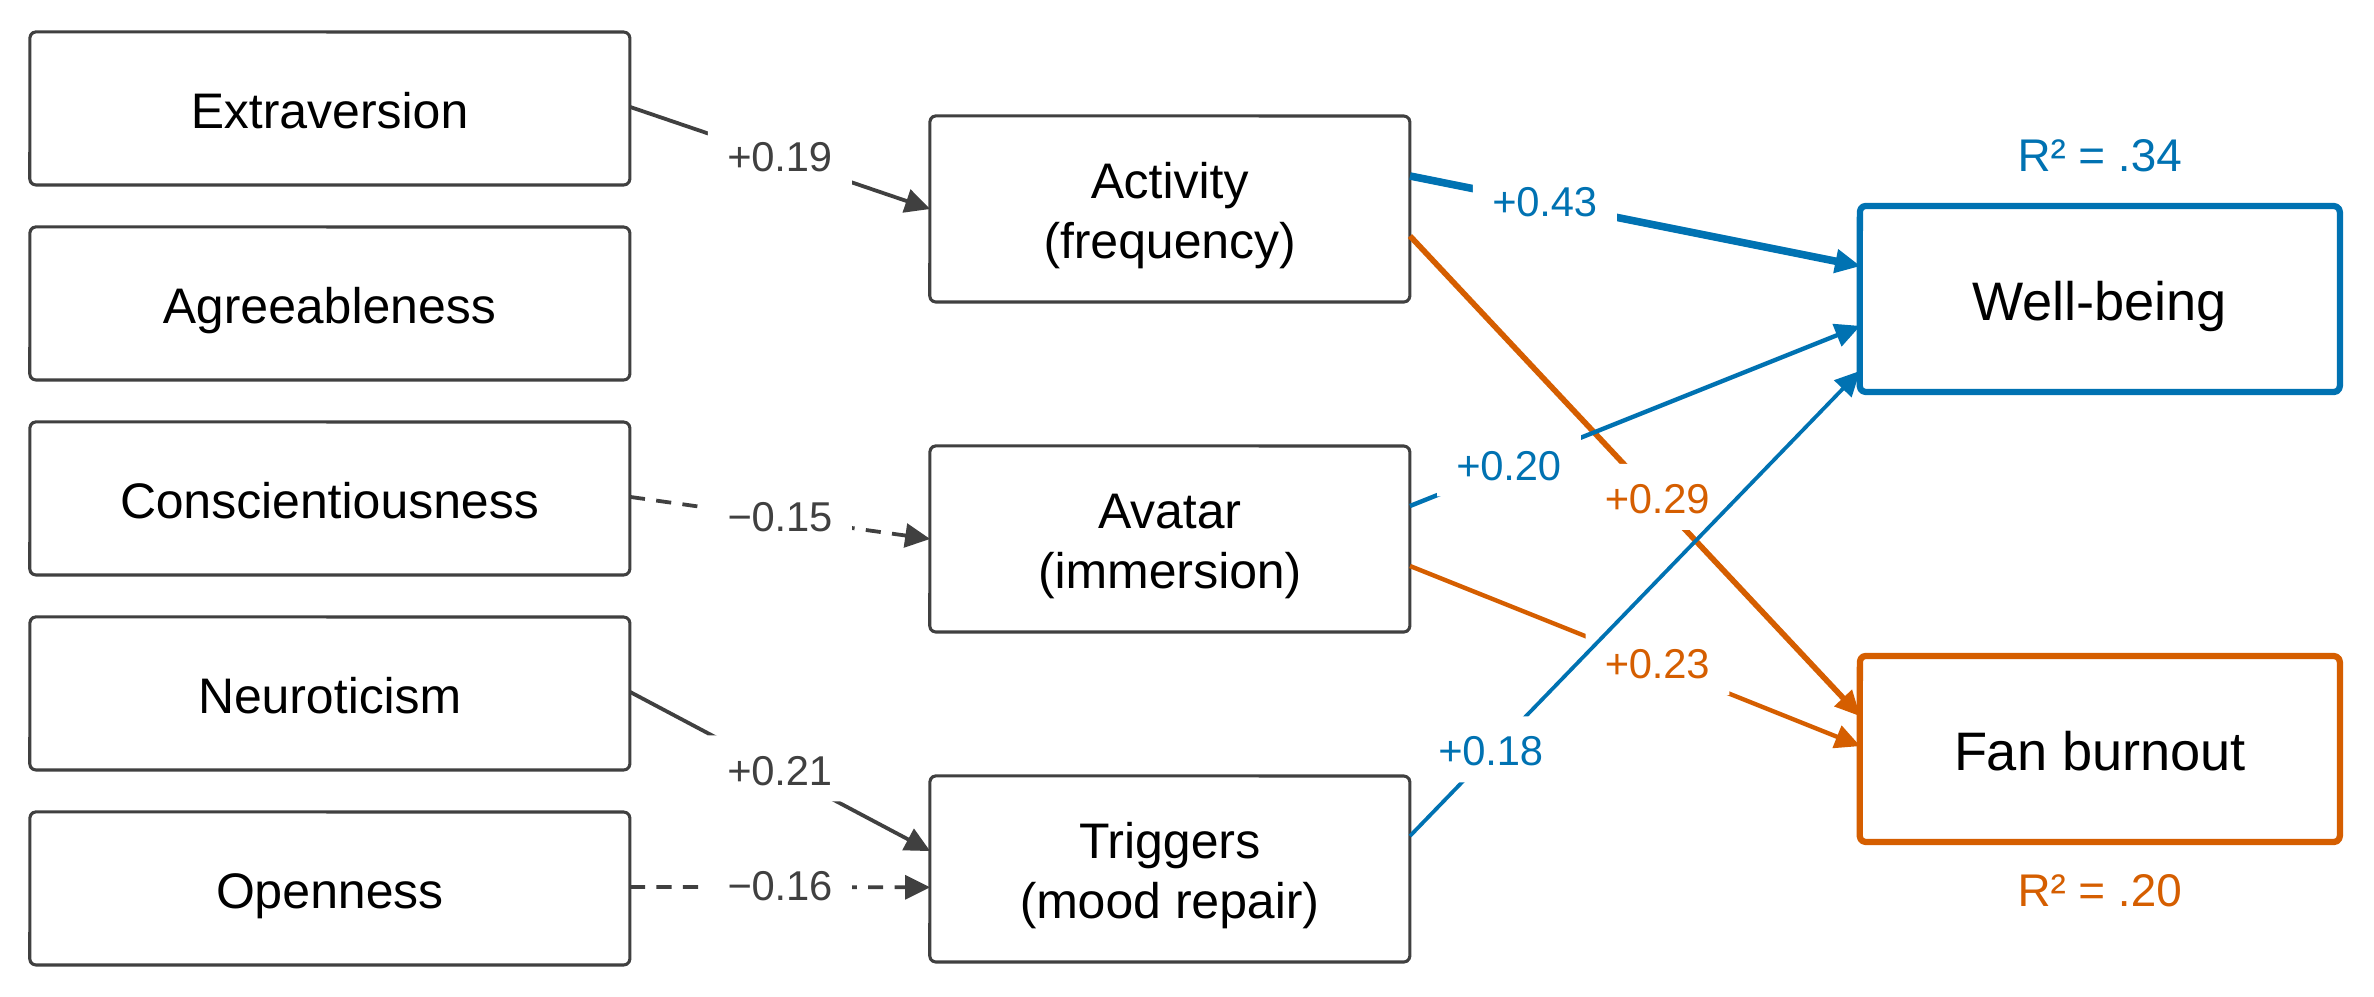
\includegraphics[width=0.85\linewidth]{figures/fig3_paths_ppt.png}
\jecaption{パスモデルの結果（$N=215$，標準化係数，$p<.05$のみ表示，破線は負の関係．青は幸福度へ，橙は推し疲れへの経路．協調性には有意な経路がなかった）}{Path model ($N=215$; standardised, $p<.05$ only; dashed = negative)}
\label{fig:paths}
\end{figure}

\begin{table}[t]
\centering
\jetcaption{パスモデルの主な標準化係数}{Main standardised coefficients of the path model}
\label{tab:paths}
\small
\begin{tabular}{@{}llrl@{}}
\toprule
説明変数 & 目的変数 & $\beta$ & 有意性 \\
\midrule
推し活の頻度 & 幸福度 & .43 & $p<.001$ \\
推し活の頻度 & 推し疲れ & .29 & $p<.001$ \\
推し活への没入 & 幸福度 & .20 & $p<.001$ \\
推し活への没入 & 推し疲れ & .23 & $p<.001$ \\
気分の回復のための推し活 & 幸福度 & .18 & $p=.003$ \\
気分の回復のための推し活 & 推し疲れ & -- & $p=.47$（n.s.） \\
\midrule
外向性 & 推し活の頻度 & .19 & $p<.05$ \\
誠実性 & 推し活への没入 & $-.15$ & $p<.05$ \\
神経症傾向 & 気分の回復のための推し活 & .21 & $p<.05$ \\
開放性 & 気分の回復のための推し活 & $-.16$ & $p<.05$ \\
\midrule
\multicolumn{4}{@{}l}{決定係数：幸福度 $R^2=.34$，推し疲れ $R^2=.20$} \\
\bottomrule
\end{tabular}
\end{table}

\subsection{RQ1b：性格は推し活の関わり方を形づくる}
性格特性は，推し活の関わり方と関連した．外向性は推し活の頻度の高さと（$\beta=.19$），誠実性は没入の低さと（$\beta=-.15$），神経症傾向は気分の回復のための推し活の多さと（$\beta=.21$），開放性はその少なさと（$\beta=-.16$）関連した．ただし，これらの効果はいずれも小さかった（$|\beta|\leq.21$）．協調性は，どの変数とも有意な関連を示さなかった．

推し活の頻度と性格5因子の交互作用項を加えても，決定係数はほとんど変化しなかった（幸福度：.344→.353，$p=.74$；推し疲れ：.196→.205，$p=.79$）．すなわち，推し活の頻度が幸福度や推し疲れに与える効果は，性格によって大きく変わるわけではなかった．

また，性格特性のみによるクラスタリングでは，シルエット係数が0.15〜0.18と低く，明確な「タイプ」には分かれなかった．3群の解では，群の間で推し疲れにわずかな差が見られた（$\eta^2=.04$，$p=.01$）．以上から，性格は単独の「タイプ」として提案に用いるよりも，行動と組み合わせて用いるのが適切であると考えられる．

\subsection{プロファイルと理想}
幸福度と推し疲れの中央値で分けた4つのプロファイルの割合を表\ref{tab:profiles}に示す．両方高い人が27\%，幸福度が高く推し疲れが低い充実型が22\%，幸福度が低く推し疲れが高い負担型が21\%，両方低い控えめ型が31\%であった．

\begin{table}[t]
\centering
\jetcaption{幸福度と推し疲れによる4つのプロファイル}{Four profiles by well-being and burnout}
\label{tab:profiles}
\small
\begin{tabular}{@{}llll@{}}
\toprule
プロファイル & 幸福度 & 推し疲れ & 割合 \\
\midrule
両方高い & 高い & 高い & 27\% \\
充実型 & 高い & 低い & 22\% \\
負担型 & 低い & 高い & 21\% \\
控えめ型 & 低い & 低い & 31\% \\
\bottomrule
\end{tabular}
\end{table}

理想と現在の頻度の差を見ると，39\%が現地イベントを，36\%がグッズの購入を「増やしたい」と回答し，「減らしたい」と回答したのはそれぞれ1\%と5\%にとどまった．最も多く「減らしたい」と回答された活動はSNSであった（22\%）．すなわち，多くのファンは推し活を全体として減らしたいわけではなく，増やしたい活動と整えたい活動が混在していた．

\subsection{RQ1c：個人の予測の精度}
性格・行動・きっかけを組み合わせた線形の予測モデルの交差検証決定係数は，幸福度で.27（RMSE 0.71），推し疲れで.11（RMSE 0.92）であった．また，ある1つの活動の頻度を1段階変えたときの予測値の変化は0.1〜0.2点にとどまり，予測の誤差よりも小さかった．すなわち，個人の幸福度と推し疲れの予測には大きな不確かさが伴う．

\section{考察}
本調査の結果，推し活の便益と負担は同じ行動（頻度と没入）から生じていることが示された．このことは，推し活に対して一律に「減らす」助言を行うと，負担だけでなく幸福度も下げてしまう可能性が高いことを意味する．また，多くのファンが現地イベントやグッズを増やしたいと考えている一方で，SNSについては減らしたいと考える人が一定数いたことから，推し活全体ではなく，本人にとって負担となっている特定の関わり方（例えば，深夜のSNS閲覧や他のファンとの比較）を整えることが支援の方向性として適切であると考えられる．

性格特性は，推し活の関わり方（どのくらい活動するか，どのくらい没入するか，気分の回復のために推し活をするか）と関連していたが，行動の効果を調整していなかった．また，性格だけでは明確なタイプに分かれなかった．このことから，性格を「あなたは○○タイプだから△△をすべき」という固定的な処方に用いるのではなく，本人の行動や負担の状況と組み合わせ，複数の提案の中から本人に合いやすいものを優先する手がかりとして用いるのが適切である．

予測の精度が限られていたことは，個人の見込みを点の値だけで示すと過信を招くおそれがあることを示している．見込みは幅とともに示し，差が小さい場合には「ほぼ同じ」と伝えるなど，不確かさを正直に示す必要がある．

本調査には限界もある．回答者は大学の連絡網を通じて募集した若年層が中心であり，推し活を行う人全体を代表しているとは限らない．TIPI-Jを5件法で用いたこと，一部の合成得点の信頼性係数が低かったこと（推し活の頻度$\alpha=.43$など）にも留意が必要である．また，横断的な調査であるため，示された関連は因果関係を意味しない．

\section{システムの設計指針}
以上の結果から，次の4つの設計指針を導いた．

\begin{description}
\item[D1：一律に減らす助言をしない．]便益と負担は同じ行動から生じるため，推し活を一律に減らす助言は行わない．「今のまま」を常に有効な選択肢として示す．
\item[D2：性格と行動を組み合わせて個人化する．]性格を固定的なタイプとして扱わず，本人の行動と負担の状況を主な手がかりとし，性格は提案の優先順位を決める補助として用いる．
\item[D3：便益と負担を同時に示す．]幸福度と推し疲れの両方を示し，提案による変化のトレードオフも示す．
\item[D4：不確かさを正直に示す．]見込みは幅とともに示し，得点の算出式と使用項目を開示する．
\end{description}

第4章では，これらの設計指針に基づいて構築したOshiFitについて述べる．

\chapter{OshiFitの設計と実装}
本章では，第3章で導いた設計指針D1〜D4に基づいて構築したシステムOshiFitについて述べる．まずシステムの全体像と利用の流れを示し，続いて質問紙，得点の算出，群の振り分け，提案の選択，プランA・Bの見込み，アバターの生成，週ごとの振り返り，データ管理，安全への配慮，実装の順に述べる．

\section{システムの概要}
OshiFitは，利用者の性格特性と推し活の状況を質問紙で把握し，推し活の状態を6つの軸で可視化したうえで，本人に合った推し活の整え方（プラン）を提案するWebアプリケーションである．利用者は，プランを取り入れなかった場合（プランA：現在のままの推し活）と取り入れた場合（プランB：最適化された推し活）の6週間後の見込みを，本人に似たアバターと数値で見比べ，どちらにするかを自分で選ぶ．選んだ後は，6週間にわたって週1回の振り返りを行い，プランの実行状況と推し疲れの変化を記録する．

OshiFitの特徴は次の4点である．
\begin{enumerate}
\item 一律に減らす助言をせず，「今のまま」も常に選べる（D1）．
\item 本人の行動と負担の状況に合わせてプランを選び，性格は優先順位の調整に用いる（D2）．
\item 幸福度と推し疲れを6つの軸で同時に示し，算出式も開示する（D3，D4）．
\item 見込みを80\%の幅とともに示し，差が小さいときは「ほぼ同じ」と伝える（D4）．
\end{enumerate}

\section{利用の流れ}
表\ref{tab:flow}に，OshiFitの利用の流れを示す．

\begin{table}[t]
\centering
\jetcaption{OshiFitの利用の流れ}{User flow of OshiFit}
\label{tab:flow}
\small
\begin{tabular}{@{}p{0.17\linewidth}p{0.37\linewidth}p{0.38\linewidth}@{}}
\toprule
段階 & 利用者が行うこと & システムが行うこと \\
\midrule
開始時（約10分） & 説明を読んで同意し，67項目の質問紙に回答する．写真または部品を選んでアバターを作る & 6軸の得点，推し疲れ（総合），性格（ビッグファイブ），推し活の傾向を計算して表示する．算出根拠も表示する \\
振り分け & 結果を見る & 6軸のうち5軸以上が60点以上，かつWHO-5の素点が13点以上なら群A（今のままで順調）とする．それ以外はプランA・Bを表示する \\
選択 & プランAとプランBを見比べ，どちらにするかを選ぶ & プランBを選んだら群B，プランAを選んだら群Cとして記録する \\
6週間 & 群B・C：週1回以上，振り返りに答える（約2分）．群A：利用は不要 & プランの実行状況，推し疲れ4項目，推し活中の幸福感，変化の自己評価を記録する \\
6週目 & 全員が終了調査（WHO-5を含む）に答える．群B・Cは使いやすさ等にも答える & 開始時と6週目のレーダーチャートを重ねて表示する \\
\bottomrule
\end{tabular}
\end{table}

\section{質問紙}
\subsection{構成}
OshiFitの質問紙は67項目からなる（表\ref{tab:questionnaire}）．第3章の調査で用いた調査票を基に，次の点を修正した．
\begin{enumerate}
\item \textbf{頻度の聞き方}：回数ではなく，「自分の推し活全体の中で，その活動がどのくらいの割合を占めているか」を5段階（まったくしない〜中心）で尋ねる形にした．推し活の量は人によって大きく異なるため，絶対的な回数よりも本人の中での相対的な比重の方が，提案の手がかりとして解釈しやすいと考えたためである．
\item \textbf{選択肢の向きの統一}：第3章の調査では回答の向きの取り違えが起きたため，すべての項目で「数字が大きいほど多い・強い」向きにそろえた．
\item \textbf{金額の聞き方}：収入に対する予算の割合は欠損が多かったため，1か月あたりの金額の区分で尋ねる形にした．
\item \textbf{TIPI-J}：第3章と同じ文言を5件法で用いた\cite{oshio2012}．
\item \textbf{WHO-5の追加}：開始時と6週目の精神的健康を比較するため，WHO-5（5項目）\cite{topp2015,inagaki2013}を追加した．
\item \textbf{主たる推しの定義}：「いま最も時間を使っている推しを1人・1組」と明記した．
\item \textbf{注意確認項目}：データの品質確認のため残した．
\end{enumerate}

\begin{table}[t]
\centering
\jetcaption{OshiFitの質問紙の構成（全67項目）}{Structure of the OshiFit questionnaire (67 items)}
\label{tab:questionnaire}
\small
\begin{tabular}{@{}p{0.3\linewidth}p{0.38\linewidth}p{0.22\linewidth}@{}}
\toprule
区分 & 項目 & 回答形式 \\
\midrule
基本情報 & Q1〜Q6（年齢，性別，職業，推しのジャンル，応援期間，1か月の金額の区分） & 選択 \\
性格（TIPI-J） & Q7〜Q16 & 5件法 \\
推し活の内容（割合） & Q17〜Q28（音楽，動画，ライブ，CD，グッズ，テレビ・ラジオ，雑誌，SNSのチェック，SNSでの発信，聖地巡礼，ファンクラブ，コラボカフェ） & 5段階 \\
気持ちと生活の変化 & Q29〜Q54（充実，生活管理，能力，交流，負担．注意確認Q42を含む） & 7件法 \\
推し活をしたくなるとき & Q55〜Q61（逃避，孤独，ご褒美，回復，SNSの影響，習慣，気分の高揚） & 7件法 \\
WHO-5 & W1〜W5（最近2週間） & 6件法（0〜5） \\
自由記述 & Q62（任意） & 記述 \\
\bottomrule
\end{tabular}
\end{table}

全項目は付録Aに示す．

\subsection{件法の選択}
気持ちと生活の変化，推し活をしたくなるときの項目は7件法とした．これらは推し活の便益と負担の微妙な程度の違いを捉える必要があり，また第3章の調査との比較のためである．一方，推し活の内容は「割合」を尋ねるため，「まったくしない」「ごく一部」「一部」「大きな部分」「中心」の5段階とした．性格は第3章と同じく5件法とした．件法は項目の性質に応じて選んでおり，すべてを統一することはしていない．

\section{6軸の得点}
OshiFitは，質問紙の回答から推し活の状態を6つの軸で0〜100点に換算し，レーダーチャートで示す（表\ref{tab:axes}）．すべての軸は外側ほど良好になるようにそろえた．負担を表す軸（睡眠・生活，お金，義務感・人間関係，SNS・比較）は，負担の項目の平均を逆にして，点数が高いほど負担が少ないことを表す．画面には，各軸の算出式と，その計算に使った本人の回答も表示する（D4）．

\begin{table}[t]
\centering
\jetcaption{6軸の得点と推し疲れ（総合）の算出式}{Formulas for the six axes and overall burnout}
\label{tab:axes}
\small
\begin{tabular}{@{}p{0.22\linewidth}p{0.2\linewidth}p{0.48\linewidth}@{}}
\toprule
軸 & 使用項目 & 算出式 \\
\midrule
幸福度 & W1〜W5 & WHO-5の合計（0〜25）$\times4$ \\
推し活の充実 & Q29〜Q34，Q39 & （7項目の平均$-1$）$\div6\times100$ \\
睡眠・生活 & Q44，Q50 & $100-$（2項目の平均$-1$）$\div6\times100$ \\
お金 & Q45，Q46 & $100-$（2項目の平均$-1$）$\div6\times100$ \\
義務感・人間関係 & Q47，Q49 & $100-$（2項目の平均$-1$）$\div6\times100$ \\
SNS・比較 & Q48，Q51 & $100-$（2項目の平均$-1$）$\div6\times100$ \\
\midrule
推し疲れ（総合） & Q44〜Q51 & （8項目の平均$-1$）$\div6\times100$（高いほど推し疲れ） \\
\bottomrule
\end{tabular}
\end{table}

\section{群の振り分け}
6軸のうち5軸以上（約8割）が60点以上，かつWHO-5の素点が13点以上の利用者には，「今の推し活は順調です」と伝え，プランは提示しない（群A）．60点は7件法で「どちらともいえない」より良い側に入る点であり，WHO-5の13点は精神的健康が良好であるとされる目安である\cite{topp2015}．すでに良好な人に変更を勧めないことは，設計指針D1に基づく．

\section{プランの選択}
群Aに当てはまらない利用者には，11種類のプランの中から3案を提示する（表\ref{tab:plans}）．各プランは，6軸のうちいずれか1つの改善を狙うものであり，第3章の結果（便益と負担が同じ行動から生じること，SNSを減らしたい人が一定数いること）に基づき，活動そのものをやめるのではなく，関わり方を整える内容とした．

\begin{table}[t]
\centering
\jetcaption{OshiFitの11種類のプラン}{Eleven plans in OshiFit}
\label{tab:plans}
\small
\begin{tabular}{@{}p{0.15\linewidth}p{0.42\linewidth}p{0.17\linewidth}p{0.14\linewidth}@{}}
\toprule
対象の軸 & プラン & 想定改善量（点） & 優先する性格 \\
\midrule
睡眠・生活 & SNSは23時まで．そのあとはお休みモード & 16 & -- \\
睡眠・生活 & リアタイは週2回まで，ほかはアーカイブで & 12 & 誠実性 \\
お金 & 今月のグッズ予算を先に決める & 16 & 誠実性 \\
お金 & 欲しいグッズは1日おいてから決める & 12 & 神経症傾向 \\
義務感 & 今週追うものを3つに絞る & 15 & -- \\
義務感 & 「行かない回」を1つ決めておく & 12 & 誠実性 \\
SNS・比較 & 比べてしまう言葉をミュートする & 15 & 神経症傾向 \\
SNS・比較 & SNSを見るのは1日2回・各15分まで & 12 & 外向性（低） \\
推し活の充実 & 友達と同時視聴の日をつくる & 12 & 外向性 \\
推し活の充実 & 感想メモや創作で推しを残す & 12 & 開放性 \\
推し活の充実 & 寝る前15分は推しの曲だけの時間 & 10 & 協調性 \\
\bottomrule
\end{tabular}
\end{table}

プランは次の手順で選ぶ．まず，6軸を点数の低い順に並べ，点数の低い軸に対応するプランほど優先する．同じ程度の優先度のプランの間では，利用者の性格の傾向に合うプランを優先する（例：誠実性が高い人には予算を先に決めるプラン，神経症傾向が高い人には比較の言葉をミュートするプラン）．3案の対象の軸が重ならないようにし，利用者が異なる方向の提案を比較できるようにする．各プランには，具体的な実行方法（例：「通知を23時にオフにし，翌朝まとめて見る」）と，選ばれた理由（例：「睡眠・生活が33点」）を表示する．これは，推薦の理由を示すことで利用者が提案を自ら評価して選べるようにするためである\cite{tintarev2007}．また，小さく実行しやすい行動を具体的な手順とともに示すことは，行動変容の理論\cite{fogg2009}とも整合する．

プランの選択は決定的な規則で行い，機械学習による学習は行わない．これは，検証実験の期間中に参加者ごとに提案の仕組みが変わらないようにし，提案の根拠を利用者と研究者の双方が確認できるようにするためである．

\section{プランAとプランBの見込み}
\subsection{見込みの算出}
プランAは，現在の回答から計算した6軸の得点をそのまま用いる．プランBは，選んだプランが対象の軸を一定の点数（v1.0ではプランごとに10〜16点，表\ref{tab:plans}）改善し，幸福度がその4分の1だけ上がると仮定して算出する．この想定改善量は，第3章の結果（推し活の頻度を1段階変えたときの予測値の変化）と，プランの実行しやすさを踏まえて設定した暫定的な値であり，検証実験の期間中はv1.0に固定する．

\subsection{不確かさの表示}
第3章の結果から，個人の予測には大きな誤差が伴うことが分かった．そこでOshiFitでは，各軸に$\pm15$点，幸福度に$\pm12$点の幅を80\%の幅の目安として表示する（D4）．幅は，前研究の予測誤差に基づいて設定した．予測の不確かさを可視化することで利用者がより適切な判断を行えることは，Kayら\cite{kay2016}の研究でも示されている．また，プランAとプランBの差が5点未満のときは「ほぼ同じ」と表示し，わずかな差を過大に受け取らないようにする．画面には「この見込みは将来を決めるものではなく，診断でもありません．今のままを選ぶこともできます」と明記する．

図\ref{fig:twofutures}に，2つの未来の表示の例を示す．

\begin{figure}[t]
\centering
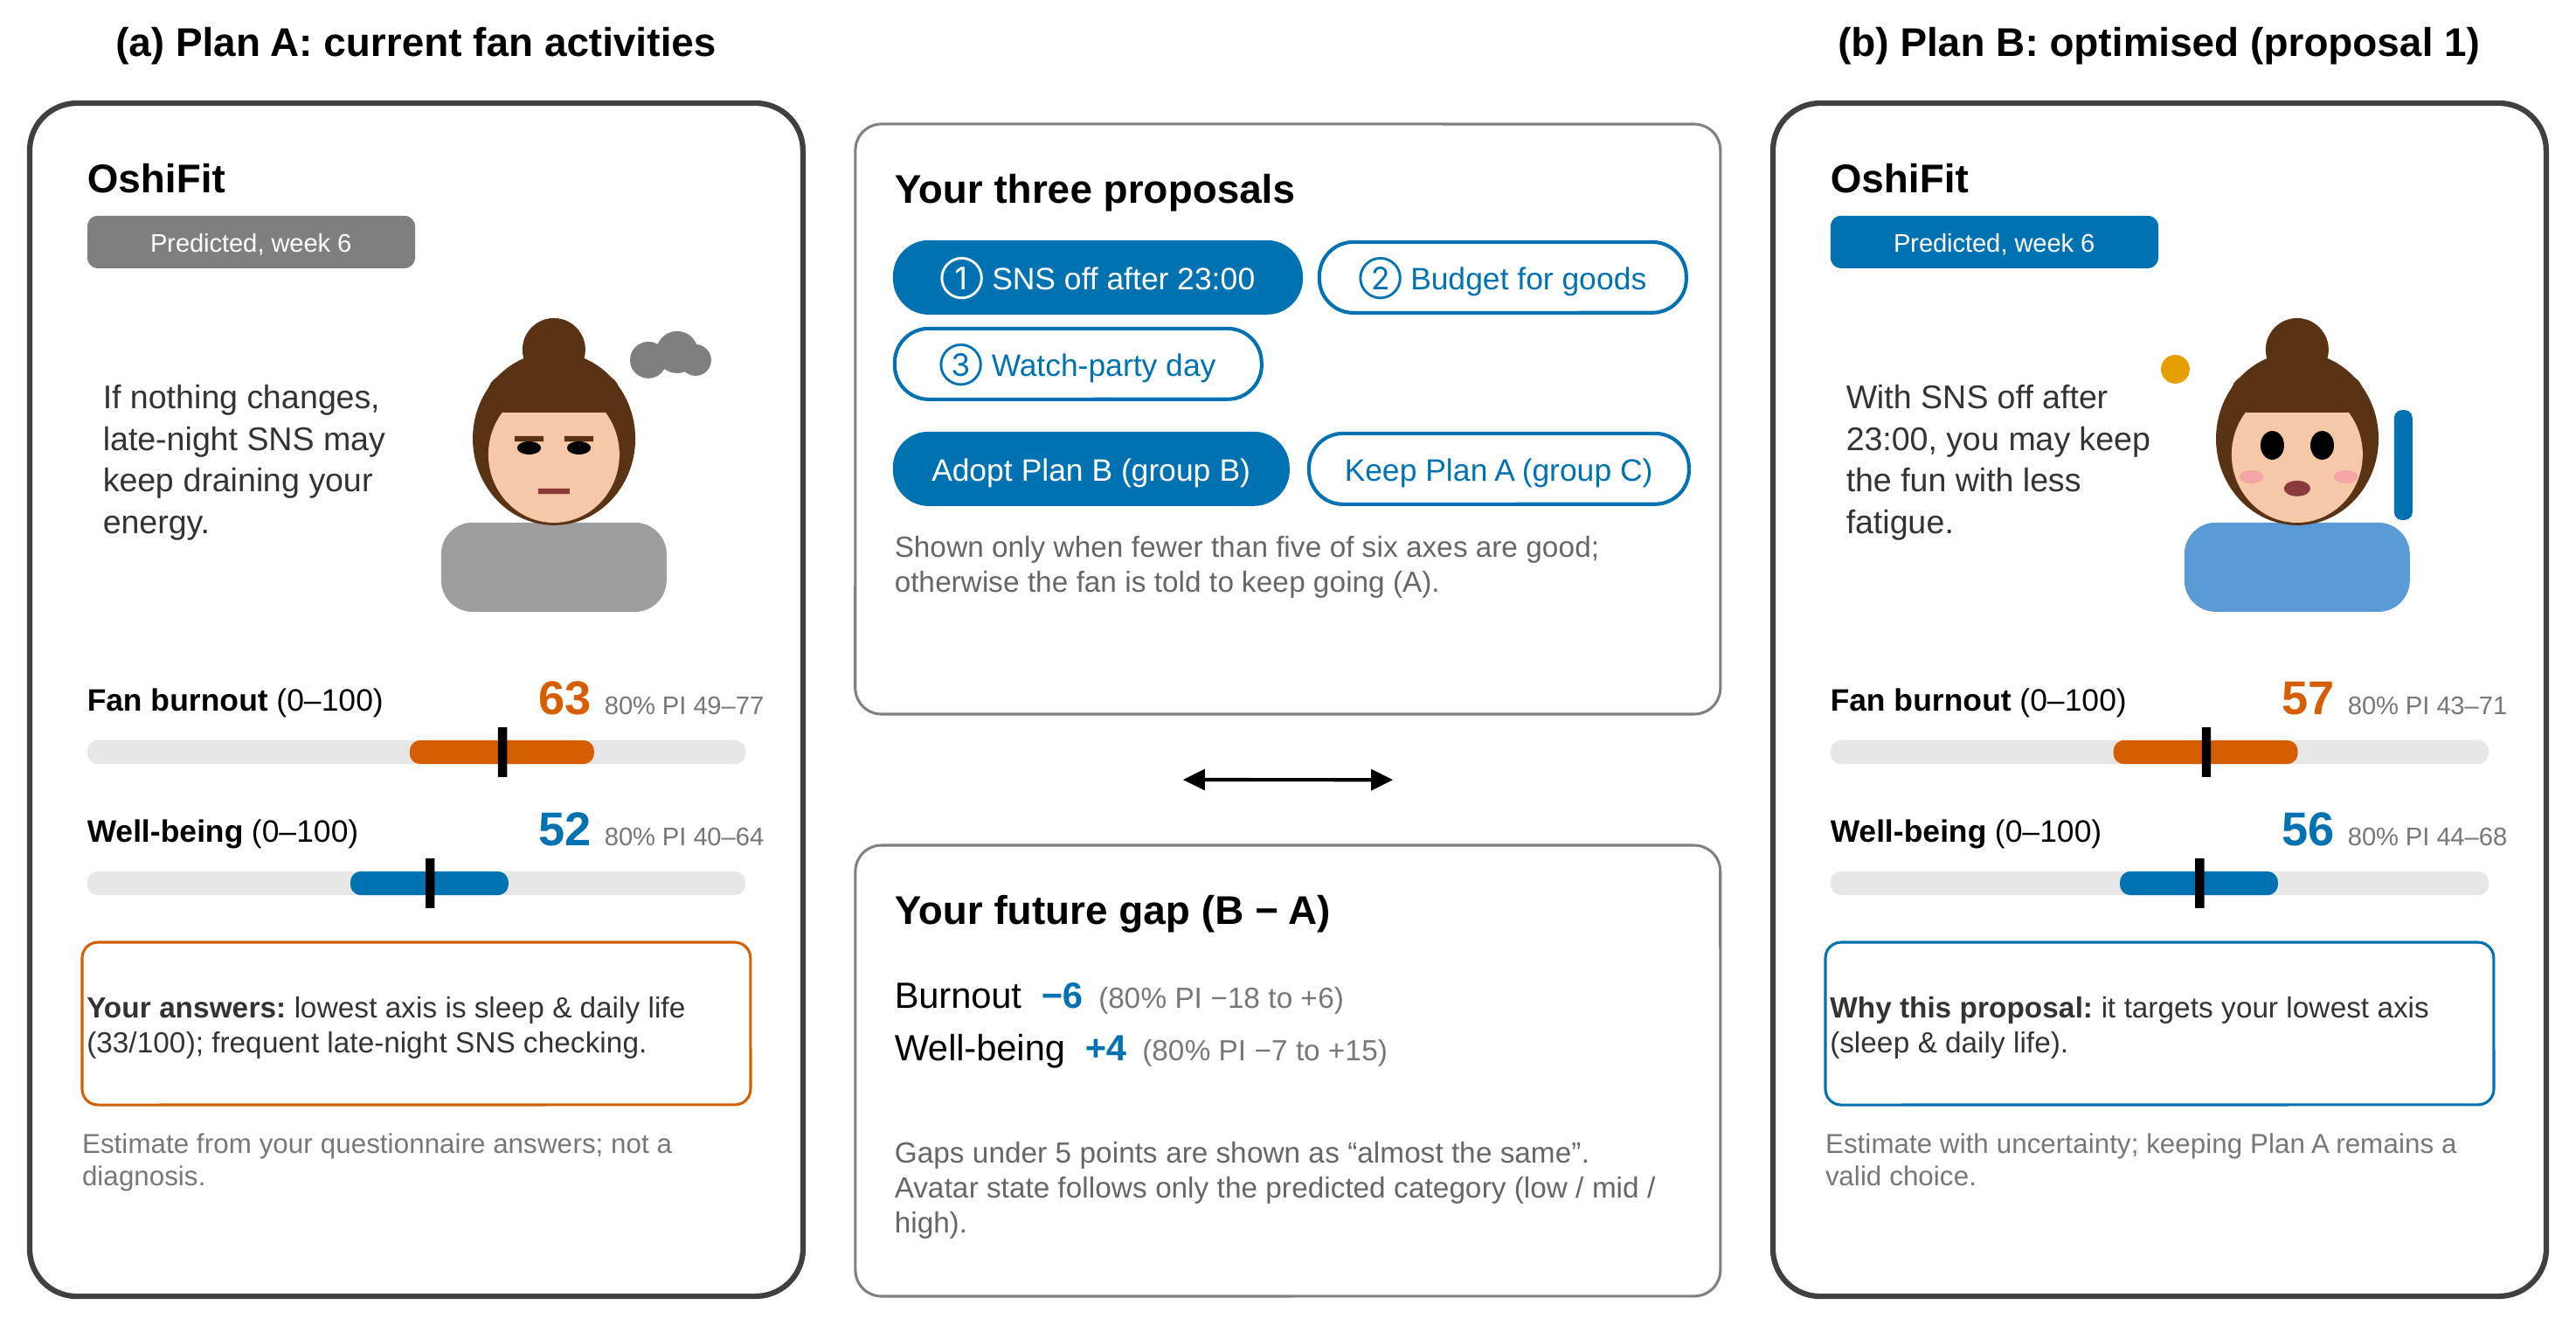
\includegraphics[width=\linewidth]{figures/fig2_twofutures_ppt.png}
\jecaption{OshiFitの「2つの未来」の表示（架空の利用者の例）．プランA（現在のままの推し活）とプランB（最適化された推し活）の6週間後の推し疲れと幸福度の見込みを80\%の幅とともに示す}{OshiFit's two-futures display (illustrative user)}
\label{fig:twofutures}
\end{figure}

\section{アバターの生成}
OshiFitでは，本人に似た2Dアバターで状態を表す．これは，本人に似た姿で将来の状態を見せることが行動のきっかけになりうるという，プロテウス効果や将来の自己に関する研究\cite{yee2007,fox2009,hershfield2011}に基づく．

アバターは，利用者が撮影または選択した顔写真から，端末の中で作成する．Googleが提供するMediaPipe\cite{lugaresi2019}の顔の特徴点検出を端末内で動かし，顔の幅と高さの比（顔の形），目の開き，眉の傾き，口の幅を測ってアバターの部品に反映する．肌と髪の色も写真から読み取る．写真と特徴点は端末の外に送らず，読み取り後すぐに破棄し，保存するのは部品の番号だけである．写真を使いたくない利用者は，部品を自分で選んでアバターを作ることもできる．

アバターの表情は，6軸の平均点の区分だけで決まる．平均が50点未満なら疲れ気味，50〜64点ならふつう，65点以上なら元気な表情とする．数値の区分に対応させ，大げさな表現は行わない．プランAとプランBのアバターは，それぞれの見込みの区分に応じた表情で並べて表示する．

\section{週ごとの振り返り}
群Bと群Cの利用者は，6週間にわたり週1回以上，振り返りに回答する（約2分）．振り返りでは，(1)プランを実行したか（行った・一部行った・行わなかった），(2)推し疲れの4項目，(3)推し活中の幸福感，(4)ストレスと幸福感の変化の自己評価を尋ねる．\todo{要確認：振り返り項目の最終版の文言（付録C）}

群Bで，プランを「行った」または「一部行った」週のうち，ストレスが「減った」かつ幸福感が「下がっていない」週は，正解データとしてアプリ内で自動的に印を付ける．この正解データは，検証実験の終了後にプランの想定改善量を更新するために用いる（5.7.6節）．

連絡先を集めない代わりに，毎週の振り返りと6週目の調査の日を，端末内で作成したカレンダー用ファイル（.ics）でカレンダーに追加できるようにした．

\section{データ管理と開発者ページ}
研究データは，Googleのクラウドサービス Firebase で一元管理する．データベース（Cloud Firestore）は東京リージョン（asia-northeast1）に置き，利用者は匿名認証で識別する．氏名や連絡先などの個人を特定できる情報は収集しない．利用者のデータは参加ID（匿名）ごとに保存し，セキュリティルールにより本人の記録だけを読み書きできるようにした．

研究者が全データを確認するための開発者ページ（admin.html）を用意し，閲覧できるのは本人（筆者）と指導教員のGoogleアカウントだけとした．開発者ページでは，参加者ごとの群，開始時の得点，週ごとの振り返り，6週目の結果を一覧でき，分析用にCSV形式で書き出せる．

\section{安全と参加者の負担への配慮}
推し活という本人にとって大切な趣味を扱うため，次の配慮を行った．
\begin{enumerate}
\item \textbf{相談先の表示}：開始時または6週目のWHO-5の素点が7点以下のとき，また週の振り返りで推し疲れ4項目の平均が6以上の週が2週続いたとき，相談先（学生相談室，厚生労働省「まもろうよ こころ」）を表示し，振り返りを休んでよいことを伝える．
\item \textbf{選択の尊重}：プランAを選ぶことも正当な選択として扱い，どちらを選んでも同じように振り返りを依頼する．
\item \textbf{参加の取りやめ}：マイページに参加ID（匿名）と「参加をやめる（記録を削除）」を表示し，押すとサーバー上と端末内の記録を削除する．
\item \textbf{写真の扱い}：写真と顔の特徴点は端末の外に送らず，保存しない．
\end{enumerate}

\section{実装}
OshiFitは，スマートフォンのブラウザで動作するWebアプリケーションとして実装した．画面はHTML，CSS，JavaScriptで作成し，Firebase Hosting で公開した．質問紙の項目と得点の算出規則はJSON形式の設定ファイルにまとめ，画面に表示する算出式と実際の計算が一致するようにした．アバターの生成にはMediaPipe Face Landmarker\cite{lugaresi2019}のWeb版を用いた．利用画面は，ホーム，分析，未来，マイページの4つのタブで構成し，質問紙への回答が終わって群が決まるまでは分析・未来のタブを表示しないようにした．また，一度選んだ群は変更できないようにした．

図\ref{fig:screens}に，OshiFitの主な画面を示す．

\begin{figure}[t]
\centering
\placeholderfig{70mm}{【要差し替え】OshiFitの画面のスクリーンショット（左から：質問紙，分析（6軸のレーダーチャートと算出根拠），未来（プランA・B），振り返り）\\ 公開版 https://oshifit-study.web.app から撮影して挿入する}
\jecaption{OshiFitの主な画面}{Main screens of OshiFit}
\label{fig:screens}
\end{figure}

本章では，OshiFitの設計と実装について述べた．第5章では，OshiFitの有用性を検証するために行う6週間の検証実験について述べる．

\chapter{検証実験（RQ2・RQ3）}
本章では，OshiFitの有用性を検証するために行う6週間の検証実験について述べる．実験の目的と仮説，倫理的配慮，参加者，群の定義，手続き，測定項目，分析計画を述べた後，結果と考察を示す．\todo{実験実施後に5.8節・5.9節を記入する}

\section{目的と仮説}
本実験の目的は，RQ2「6週間の利用で，すでに良好な人（群A），プランBを選んだ人（群B），プランAを選んだ人（群C）の幸福度と推し疲れは，それぞれの群の中でどう変化し，群の間でどう異なるか」と，RQ3「利用者は自分の推し疲れの原因に気づき，特に行動を変えた人はシステムを有用と評価するか」に答えることである．次の仮説を立てる．

\begin{description}
\item[H1] 群Bでは，開始時に比べて6週目の推し疲れが低下し，幸福度（WHO-5）が維持または向上する．
\item[H2] 開始時の状態と性格を調整したうえで，群Bは群Cに比べて6週目の推し疲れが低く，幸福度が高い．
\item[H3] 群Bの中で，プランを実行した程度が高い人ほど，推し疲れの低下が大きい（用量反応関係）．
\item[H4] 群Bと群Cの利用者の多くが，OshiFitによって自分の推し疲れの原因に気づいたと回答し，特に群Bの利用者はOshiFitを有用と評価する．
\end{description}

群Aは開始時に良好な状態にある人であるため，6週間で大きな変化は想定しないが，平均への回帰によってわずかに低下する可能性がある．

\section{倫理的配慮}
本実験は，大阪工業大学の研究倫理審査の承認を得てから実施する．\todo{要記入：審査委員会の名称，承認番号，承認日}本研究は人を対象とする医学系研究には該当しないと指導教員と判断し，臨床試験の登録は行わない．

参加者には，研究の目的，内容，所要時間，データの扱い，参加の任意性と途中で取りやめられることを画面で説明し，同意を得てから開始する．氏名や連絡先などの個人を特定できる情報は収集しない．写真と顔の特徴点は端末の外に送らず，保存しない．データはFirebase（東京リージョン）に匿名の参加IDで保存し，閲覧は研究者（筆者と指導教員）に限る．参加の取りやめを選んだ参加者の記録は削除する．WHO-5や推し疲れの得点が一定の基準を下回った場合には相談先を表示する（4.11節）．実験の終了後には，全参加者に研究の目的と結果の概要を説明し（デブリーフィング），すべての機能を利用できるようにする．

\section{参加者}
推し活を日常的に行っている18歳以上の人を対象とし，大学の連絡網やSNSを通じて募集する．目標とする参加者数は約240名とした．これは，6週目までの離脱と群Aの割合を見込んだうえで，群Bと群Cの比較に必要な人数を確保するためである．\todo{要記入：実際の募集期間，募集方法，参加者数，属性，離脱者数}

\section{群の定義}
本実験では，参加者を無作為に群に割り付けることはしない．群は，開始時の状態と本人の選択によって決まる．
\begin{description}
\item[群A（すでに良好）] 開始時に6軸のうち5軸以上が60点以上，かつWHO-5の素点が13点以上の人．プランは提示せず，6週目に再度回答してもらう．
\item[群B（プランBを選択）] 群Aに当てはまらず，2つの未来を見比べたうえでプランBを選んだ人．
\item[群C（プランAを選択）] 群Aに当てはまらず，2つの未来を見比べたうえでプランA（今のまま）を選んだ人．
\end{description}

無作為化を行わない理由は，趣味である推し活に対して，研究の都合で変更を強制したり禁止したりすることが，設計指針D1（「今のまま」を常に有効な選択肢とする）に反するためである．その代わりに，群の差を解釈する際には，開始時の状態と性格による違いを統計的に調整し，結果は効果ではなく「関連」として解釈する．

\section{手続き}
\begin{enumerate}
\item \textbf{開始時（約10分）}：参加者は説明を読んで同意し，67項目の質問紙に回答し，アバターを作成する．OshiFitは6軸の得点とその算出根拠を表示し，群を判定する．
\item \textbf{選択}：群Aに当てはまらない参加者は，3つのプランとプランA・Bの見込みを見て，プランBを選ぶか，プランAを選ぶかを決める．
\item \textbf{6週間}：群Bと群Cの参加者は，週1回以上，振り返りに回答する（約2分）．群Aの参加者は，期間中の利用は不要とする．
\item \textbf{6週目}：全員がWHO-5を含む終了調査に回答する．群Bと群Cの参加者は，気づき，使いやすさ，有用性に関する項目にも回答する．
\item \textbf{終了後}：全員にデブリーフィングを行う．
\end{enumerate}

習慣の形成には個人差が大きく，数週間から数か月を要することが知られている\cite{lally2010}．本実験では，参加者の負担と修士研究の期間を考慮して6週間とし，習慣の定着ではなく，プランの実行と推し疲れ・幸福度の変化の関係を捉えることを目的とする．

\section{測定項目}
\subsection{主要な結果指標}
\begin{itemize}
\item \textbf{幸福度}：WHO-5\cite{topp2015,inagaki2013}の素点（0〜25）．開始時と6週目に測定する．
\item \textbf{推し疲れ（総合）}：Q44〜Q51の8項目から算出した0〜100点（表\ref{tab:axes}）．開始時と6週目に測定する．
\end{itemize}

\subsection{副次的な結果指標}
\begin{itemize}
\item 6軸それぞれの得点（開始時と6週目）
\item 週ごとの推し疲れ4項目と推し活中の幸福感
\item プランの実行率（行った$=1$，一部行った$=0.5$，行わなかった$=0$の6週間の平均）
\item 気づき（「OshiFitを使って，自分の推し疲れの原因に気づいた」など）
\item 使いやすさと有用性（群B・C）\todo{要確認：終了調査の項目の最終版（付録D）}
\end{itemize}

\section{分析計画}
分析の計画は，データの収集を始める前に定めた．無作為化を行わない設計における群の比較方法（共分散分析，傾向スコアによる重み付け，多重比較の補正）については，データサイエンス学科の濱田悦夫教授から統計解析に関する助言を得た．

\subsection{各群の前後比較}
各群について，開始時と6週目のWHO-5と推し疲れを，対応のある$t$検定とWilcoxonの符号順位検定で比較し，効果量$d_z$を求める．

\subsection{3群の比較}
6週目の値を目的変数とし，群，開始時の値，性格5因子を説明変数とする共分散分析（ANCOVA）を行う．群Aを基準として，群Bと群Cとの差を推定する．群Aは開始時の状態で選ばれているため，差は効果ではなく関連として解釈する．

\subsection{群Bと群Cの比較}
プランBを選ぶかどうかは本人の選択であるため，選択のしやすさに関わる要因によって群Bと群Cの間に違いが生じうる．そこで，性格，開始時の6軸・WHO-5・推し疲れ，推し活の頻度から，プランBを選ぶ確率（傾向スコア）\cite{rosenbaum1983,hoshino2009}を推定し，その逆数で重み付けした回帰によって，開始時の値を調整したうえで群Bと群Cの6週目の値を比較する．傾向スコアで調整しても測定されていない違いは残るため，結論は関連までとする．

\subsection{用量反応関係}
群Bの中で，プランの実行率と推し疲れ・幸福度の変化量の関係を回帰分析で調べる．実行率が高いほど推し疲れの低下が大きいという関係が見られれば，プランが変化に関わっていることの根拠が強まる．

\subsection{多重比較}
主要な比較（WHO-5と推し疲れ$\times$各群の前後比較と群Bと群Cの比較）には，Holm法による補正を行う．

\subsection{正解データによる想定改善量の更新}
実験の終了後に1回だけ，群Bの正解データ（プランを実行し，ストレスが減り，幸福感が下がっていない週）を用いてプランの想定改善量を更新する．プランごとに，正解データが1週以上ある参加者について狙った軸の実際の変化量（6週目$-$開始時）の平均を求め，
\begin{equation}
\text{新しい想定改善量}=\frac{10\times\text{これまでの想定改善量}+n\times\text{観測された平均}}{10+n}
\end{equation}
とする（$n$はそのプランの該当人数）．人数が少ないプランは元の値から大きく動かない．更新した値をモデルv1.1とし，研究終了後の利用に用いる．実験期間中はv1.0のまま変えない．

\section{結果}
\todo{実験実施後に記入}

\subsection{参加者の内訳}
\todo{要記入：募集人数，同意者数，6週目まで回答した人数，各群の人数と属性}

\begin{table}[t]
\centering
\jetcaption{各群の参加者の内訳と開始時の得点（実験後に記入）}{Participants and baseline scores by group (to be completed)}
\label{tab:groups}
\small
\begin{tabular}{@{}lccc@{}}
\toprule
 & 群A & 群B & 群C \\
\midrule
人数 & -- & -- & -- \\
年齢（中央値） & -- & -- & -- \\
WHO-5（開始時） & -- & -- & -- \\
推し疲れ（開始時） & -- & -- & -- \\
\bottomrule
\end{tabular}
\end{table}

\subsection{各群の前後比較（RQ2）}
\todo{要記入：表\ref{tab:prepost}に各群の開始時と6週目のWHO-5・推し疲れ，検定結果，効果量を記入}

\begin{table}[t]
\centering
\jetcaption{各群の開始時と6週目の比較（実験後に記入）}{Baseline vs.\ week 6 by group (to be completed)}
\label{tab:prepost}
\small
\begin{tabular}{@{}llccccc@{}}
\toprule
群 & 指標 & 開始時 & 6週目 & 差 & $p$（Holm） & $d_z$ \\
\midrule
A & WHO-5 & -- & -- & -- & -- & -- \\
A & 推し疲れ & -- & -- & -- & -- & -- \\
B & WHO-5 & -- & -- & -- & -- & -- \\
B & 推し疲れ & -- & -- & -- & -- & -- \\
C & WHO-5 & -- & -- & -- & -- & -- \\
C & 推し疲れ & -- & -- & -- & -- & -- \\
\bottomrule
\end{tabular}
\end{table}

\subsection{群の比較（RQ2）}
\todo{要記入：ANCOVAの結果（群Aを基準とした群B・Cの差と95\%信頼区間），傾向スコアで重み付けした群Bと群Cの比較}

\subsection{プランの実行と変化（RQ2）}
\todo{要記入：群Bのプランの実行率の分布，実行率と変化量の関係，プランごとの選ばれた回数と実行率}

\subsection{気づきと有用性（RQ3）}
\todo{要記入：気づき・使いやすさ・有用性の回答の分布，群Bと群Cの比較，自由記述の分析}

\section{考察}
\todo{実験実施後に記入：仮説H1〜H4の検証結果，予想と異なった点とその理由，正解データによる想定改善量の更新結果}

\chapter{総合考察}
本章では，第3章の調査と第5章の検証実験の結果を踏まえ，本研究で得られた知見を総合的に考察する．\todo{検証実験の結果が出たら6.2節・6.3節を中心に加筆する}

\section{推し活の便益と負担は同じ行動から生じる}
第3章の調査では，推し活の頻度と没入が，幸福度と推し疲れの両方と関連していた．また，幸福度と推し疲れは正の相関を示し，推し活によって幸福を感じている人ほど推し疲れも感じやすい傾向があった．このことは，推し活の支援において「活動を減らす」ことを目標にすると，負担だけでなく楽しさや生きがいまで失わせてしまう可能性が高いことを示している．

この知見は，一般的なデジタルウェルビーイングの支援が前提とする「減らすほど良い」という考え方とは異なる．推し活のように本人の生きがいと結びついた活動では，活動の量ではなく，負担につながる特定の関わり方（深夜のSNS閲覧，予算を決めない購入，すべてを追おうとする義務感，他のファンとの比較など）を整えることが重要である．OshiFitのプランが，活動をやめることではなく，時間帯や予算，追う範囲，見る言葉を整える内容になっているのはこのためである．

また，気分の回復のための推し活は幸福度とのみ関連し，推し疲れとは関連しなかった．つらいときに推しに支えられるという推し活の役割は，負担を伴わずに幸福を支える側面であると考えられる．寝る前に推しの曲だけを聴く時間をつくるプランなど，推し活の回復的な側面を生かすプランを含めたのはこのためである．

\section{性格特性の役割}
性格特性は推し活の関わり方と関連していたが，推し活の頻度の効果を調整してはいなかった．また，性格のみでは明確なタイプに分かれなかった．これらの結果は，性格を固定的なタイプとして扱い，タイプごとに決まった推し活を勧めるという方法が，推し活の支援には適さないことを示している．

一方で，性格は推し活の関わり方の違いを通じて，どのような負担が生じやすいかに関わっている可能性がある．例えば，神経症傾向の高い人は気分の回復のために推し活をしやすく，SNS上での比較による落ち込みを経験しやすいと考えられる．OshiFitでは，本人の負担の状況を主な手がかりとしてプランを選び，性格は同じ優先度のプランの中から本人に合いやすいものを選ぶ補助として用いた．この方法は，性格による個人化の利点を生かしつつ，性格による決めつけを避けるものである．

\todo{検証実験後に追記：性格によってプランの実行率や効果に違いがあったか}

\section{不確かさを示すことの意味}
個人の幸福度と推し疲れの予測精度は限られており，特に推し疲れの交差検証決定係数は.11にとどまった．この結果は，個人に見込みを示すシステムにとって重要な制約である．OshiFitでは，見込みを80\%の幅とともに示し，差が小さいときは「ほぼ同じ」と表示し，見込みが診断ではないことを明記した．

不確かさを示すことは，システムの説得力を弱めるように見えるかもしれない．しかし，推し活のように本人の価値観が関わる領域では，不確かな予測を確かなもののように示すことは，本人の判断を誤らせるだけでなく，システムへの信頼を損なうおそれがある．予測の幅を示し，算出式を開示し，最終的な選択を本人に委ねることで，利用者はシステムの提案を一つの材料として自ら考えることができる．

\todo{検証実験後に追記：利用者は幅のある見込みをどのように受け取ったか（自由記述など）}

\section{アバターで2つの未来を示すことについて}
OshiFitは，本人に似たアバターでプランAとプランBの見込みを並べて示した．先行研究\cite{fox2009,hershfield2011}が対象とした運動や貯蓄とは異なり，推し活には一方向の理想がない．そのためOshiFitでは，アバターに一方の未来だけを示すのではなく，今のままの未来と整えた未来を並べ，どちらも選べる形にした．また，アバターの表情は数値の区分だけで決まるようにし，大げさな表現を避けた．

\todo{検証実験後に追記：アバターの提示が選択や実行にどう関わったか．なお本研究の設計では，アバターの有無による比較は行っていないため，アバターそのものの効果は検証の対象外である}

\section{本研究の限界}
本研究には次の限界がある．

\begin{enumerate}
\item \textbf{調査対象の偏り}：第3章の調査の回答者は大学の連絡網を通じて募集した若年層が中心であり，推し活を行う人全体を代表しているとは限らない．年齢や推しのジャンルによって結果が異なる可能性がある．
\item \textbf{測定の信頼性}：TIPI-Jを原版の7件法ではなく5件法で用いたこと，また一部の合成得点（推し活の頻度など）の信頼性係数が低かったことにより，関連の大きさが過小に推定されている可能性がある．
\item \textbf{横断的なデータ}：第3章の調査は横断的であり，示された関連は因果関係を意味しない．
\item \textbf{無作為化を行わない設計}：検証実験の群は本人の状態と選択で決まるため，群の差をプランやOshiFitの効果と断定することはできない．傾向スコアと開始時の値で調整しても，測定されていない違いは残る．
\item \textbf{見込みの仮定の暫定性}：プランBの見込みに用いた想定改善量，複数の提案の倍率（0.8・0.6），提案の選び方の係数（12・18），群Aの基準（60点・5軸以上），個人補正のばらつきの値は，データから推定した値ではなく暫定的な設計上の値であり，実験の結果によって確かめ，更新する必要がある．
\item \textbf{自己報告}：幸福度と推し疲れはいずれも自己報告に基づくため，望ましく見せようとする回答の影響を受ける可能性がある．前研究のような生理指標との組み合わせは，本研究では行っていない．
\item \textbf{期間}：約28日間は，行動が習慣として定着するには短い\cite{lally2010}．当初計画の6週間から短くしたため，提案の効果が現れる前に調査が終わる可能性がある．
\item \textbf{計画からの変更}：当初の研究計画では，無作為の3群（記録のみ，文章での提案，提案とアバター）と2週間の記録だけの期間を予定していたが，D1に基づき本人の選択による群とし，記録だけの期間も設けなかった．そのため，アバターの有無による比較や，2週目の値を共変量とする分析はできない．
\item \textbf{回答の負担と欠測}：毎日のアンケートは負担が小さいように設計したが，回答しない日が生じる．混合モデルは欠けた日があっても推定できるが，回答しなかった理由が状態の悪さと関係する場合には偏りが残る．
\item \textbf{生成AIによる提案文}：提案文は利用者の推しに合わせて生成AIが書くため，同じ型でも文の具体性や分かりやすさが人によって異なる．提案ごとの分析は型の単位で行うが，その結果には文の違いの影響も含まれる．また，生成された文は研究者が事前に一つずつ確認したものではない．禁止した表現の確認と固定の文への切り替えで対処したが，すべての不適切な文を防げるとは限らない．
\item \textbf{デバッグ協力者の参加}：システムのデバッグに協力した研究室の院生が本実験に参加した場合，提案の内容や研究の狙いを事前に知っている．本分析から除いた結果も示すが，完全には取り除けない．
\end{enumerate}

\section{社会的な意義}
本研究は，推し活という多くの人が日常的に行っている活動を対象に，それをやめさせるのではなく，本人が楽しみを保ちながら負担を減らせるよう支援する方法を示した．推し活に限らず，ゲーム，スポーツ観戦，創作活動など，楽しさと負担が表裏一体となった趣味や娯楽は多い．本研究の設計指針（一律に減らさない，行動と性格を組み合わせて個人化する，便益と負担を同時に示す，不確かさを正直に示す）は，これらの活動を持続可能な形に整えるための支援にも応用できると考えられる．

\chapter{まとめと今後の展望}

\section{まとめ}
本研究では，個人の性格特性と日々の推し活の状況から，その人に適した推し活方法を提案するシステムOshiFitを構築し，その有用性を検証した．

第1章では，メンタル不調の増加と推し活の広がりを背景に，推し活が便益と負担の両方をもたらすこと，本人は自分の負担の原因に気づきにくいこと，先行研究には便益と負担を同時に扱った定量的な検討や個人を支援する仕組みが不足していることを述べ，3つのリサーチクエスチョンを設定した．

第2章では，推し活・ファン行動，ウェルビーイングとバーンアウト，性格特性と個人化，パーソナルインフォマティクスと行動変容，アバターと将来の自己，予測の不確かさの提示に関する先行研究を概観し，本研究の位置付けを示した．

第3章では，215名のファンを対象とした質問紙調査により，RQ1に答えた．推し活の頻度と没入は幸福度と推し疲れの両方と関連し，便益と負担が同じ行動から生じることが分かった．性格特性は推し活の関わり方と関連したが，行動の効果を調整してはおらず，性格だけでは明確なタイプに分かれなかった．個人の予測の精度は限られていた（交差検証決定係数：幸福度.27，推し疲れ.11）．これらの結果から，一律に減らす助言をしない（D1），性格と行動を組み合わせて個人化する（D2），便益と負担を同時に示す（D3），不確かさを正直に示す（D4）という4つの設計指針を導いた．

第4章では，設計指針に基づいてOshiFitを設計・実装した．OshiFitは67項目の質問紙から6軸の得点を算出して算出式とともに示し，すでに良好な人には今のままでよいことを伝え，それ以外の人には11種類のプランから3案を示す．さらに，プランAとプランBの6週間後の見込みを幅とともに本人に似たアバターで示し，本人が選んだうえで6週間の振り返りを支援する．

第5章では，RQ2とRQ3に答えるための6週間の検証実験の方法と分析計画を述べた．\todo{実験後に記入：主な結果}

第6章では，便益と負担が同じ行動から生じることの意味，性格特性の役割，不確かさを示すことの意味，アバターで2つの未来を示すことについて考察し，本研究の限界を述べた．

\section{今後の展望}
今後の展望として，次の点が挙げられる．

\begin{enumerate}
\item \textbf{対象の拡大}：年齢層や推しのジャンル（アイドル，キャラクター，VTuber，スポーツ選手など）をより幅広く含めた調査を行い，知見の一般化を図る．
\item \textbf{想定改善量の更新と予測の改善}：検証実験で得られた正解データにより想定改善量を更新し（モデルv1.1），利用者が増えるにつれて予測の精度を高める．週ごとの振り返りのデータを用いた，個人内の変化を捉える予測モデルも検討する．
\item \textbf{アバターの効果の検証}：本研究ではアバターの有無による比較を行っていない．今後は，アバターで見込みを示す場合と文章や数値だけで示す場合を比較し，アバターそのものの効果を検証する．
\item \textbf{生理指標との組み合わせ}：前研究で用いたスマートウォッチによる心拍変動\cite{thayer2007}などの生理指標を組み合わせ，自己報告だけでは捉えにくいストレスの変化を捉える．
\item \textbf{長期的な効果}：6週間より長い期間の利用で，プランが習慣として定着するか，推し疲れの低下が持続するかを検証する．
\item \textbf{社会実装}：研究で構築したOshiFitを，誰もが気軽に使えるアプリケーションとして公開し，展示やファンコミュニティとの連携を通じて，推し活を持続可能な形で楽しむための支援として普及させる．
\end{enumerate}


\chapter*{謝辞}
\addcontentsline{toc}{chapter}{謝辞}
本研究を進めるにあたり，終始ご指導をいただいた大阪工業大学 大井翔先生に心より感謝申し上げます．研究の方向付けから調査・システム開発・論文執筆に至るまで，多くの助言をいただきました．また，大阪工業大学 情報科学部 データサイエンス学科 濱田悦夫教授には，データサイエンスと統計解析の観点から，調査データの分析方法（構造方程式モデリング，因果構造の探索，効果の推定）や検証実験の分析計画について貴重なご助言をいただきました．深く感謝申し上げます．また，調査に協力してくださった回答者の皆様，検証実験に参加してくださった皆様，日頃から議論に付き合ってくださったメディアインタラクション研究室の皆様に深く感謝いたします．
\todo{要記入：研究費（科研費等）や協力者があれば記載}

\bibliographystyle{junsrt}
\bibliography{references}
\addcontentsline{toc}{chapter}{参考文献}

\chapter*{研究業績}
\addcontentsline{toc}{chapter}{研究業績}
\section*{国際会議}
\begin{enumerate}
\item Gen Imai, Sho Ooi: ``OshiFit: Study on Proposal System with `Oshi-katsu' based on Individual Characteristics Predicted by One's Own Avatar,'' IEVC 2026（ポスター発表）．
\item Gen Imai, Sho Ooi: ``OshiFit: Showing Fans Two Futures of Their Fan Activities with a Self-Resembling Avatar,'' CHIIR 2027 Short Paper（投稿中，Submission 321）．\todo{採否が決まり次第更新}
\end{enumerate}
\section*{国内学会}
\begin{enumerate}
\item 今井元，大井翔：推し活時の心拍とストレスとの関連性に関する研究，ウェルビーイング学会 第3回年次大会，2025．
\item 今井元，大井翔：2026年度 情報処理学会関西支部 支部大会，G-43，2026．\todo{要確認：題目}
\end{enumerate}

\appendix
\chapter{質問紙の全項目}
\label{app:questionnaire}
OshiFitで用いる質問紙（全67項目）を示す．Q42は注意確認項目である．

\section*{あなたご自身と推し活について}
\noindent 以下の質問には「主たる推し」（いま最も時間を使っている推しを1人・1組）について答えてください。\\
\begin{longtable}{@{}p{0.08\linewidth}p{0.86\linewidth}@{}}
\toprule 番号 & 項目 \\ \midrule \endhead \bottomrule \endfoot
Q1 & 年齢 \\
Q2 & 性別\newline {\footnotesize（男性，女性，その他，回答しない）} \\
Q3 & 職業\newline {\footnotesize（学生，会社員・公務員，自営業・フリーランス，パート・アルバイト，主婦・主夫，その他）} \\
Q4 & 主たる推しのジャンル\newline {\footnotesize（実在のアイドル，アニメ・漫画・ゲームのキャラクター，VTuber・配信者，俳優・舞台役者，声優，バンド・アーティスト，スポーツ選手，その他）} \\
Q5 & その推しを応援し始めてからの期間\newline {\footnotesize（半年未満，半年〜1年未満，1年〜3年未満，3年〜5年未満，5年以上）} \\
Q6 & 推し活に使う1か月あたりの金額（目安）\newline {\footnotesize（5,000円未満，5,000円〜1万円未満，1万円〜3万円未満，3万円〜5万円未満，5万円以上，答えたくない）} \\
\end{longtable}
\section*{あなた自身の性格について（TIPI-J）}
\noindent 以下の項目はどの程度当てはまりますか。直感でお答えください。\\
\noindent {\small 回答：1：全く違うと思う／2：少し違うと思う／3：どちらでもない／4：少しそう思う／5：強くそう思う}
\begin{longtable}{@{}p{0.08\linewidth}p{0.86\linewidth}@{}}
\toprule 番号 & 項目 \\ \midrule \endhead \bottomrule \endfoot
Q7 & 活発で外向的だと思う \\
Q8 & 他人に不満をもち、もめごとを起こしやすいと思う \\
Q9 & しっかりしていて、自分に厳しいと思う \\
Q10 & 心配性で、うろたえやすいと思う \\
Q11 & 新しいことが好きで、変わった考えをもつと思う \\
Q12 & 寡黙で静かだと思う \\
Q13 & 思いやりがあり、温かいと思う \\
Q14 & だらしなく、うっかりしていると思う \\
Q15 & 冷静で、気分が安定していると思う \\
Q16 & 発想力が乏しく、平凡だと思う \\
\end{longtable}
\section*{推し活の中身（割合）}
\noindent 回数ではなく、あなたの推し活全体の中で、それぞれの活動がどのくらいの割合を占めているかをお答えください。\\
\noindent {\small 回答：1：まったくしない／2：ごく一部（たまにする程度）／3：一部（いくつかある活動の一つ）／4：大きな部分（主な活動の一つ）／5：中心（推し活のほとんどがこれ）}
\begin{longtable}{@{}p{0.08\linewidth}p{0.86\linewidth}@{}}
\toprule 番号 & 項目 \\ \midrule \endhead \bottomrule \endfoot
Q17 & 推しに関係する音楽を聴いている \\
Q18 & 推しに関連する動画（YouTube、MVなど）を視聴している \\
Q19 & 推しのライブやイベントに現地参加している \\
Q20 & 推しのCDやBlu-rayなどを購入している \\
Q21 & 推しのグッズ（アクスタ、タオル等）を購入している \\
Q22 & 推しが出演するテレビ番組やラジオをチェックしている \\
Q23 & 推しに関連する雑誌や書籍を購入している \\
Q24 & 推しのSNS（X、Instagram等）をフォロー・チェックしている \\
Q25 & SNSで推しに関する情報を発信・共有している \\
Q26 & 推しの聖地巡礼（ロケ地めぐり等）を行っている \\
Q27 & ファンクラブや有料会員サービスに入会している \\
Q28 & 推しのコラボカフェやポップアップストアに行っている \\
\end{longtable}
\section*{推し活を通じた気持ちと生活の変化}
\noindent 推し活をしている中でのあなたの気持ちや生活について、どの程度当てはまりますか。\\
\noindent {\small 回答：1：全く当てはまらない／2：ほとんど当てはまらない／3：あまり当てはまらない／4：どちらともいえない／5：やや当てはまる／6：かなり当てはまる／7：非常に当てはまる}
\begin{longtable}{@{}p{0.08\linewidth}p{0.86\linewidth}@{}}
\toprule 番号 & 項目 \\ \midrule \endhead \bottomrule \endfoot
Q29 & 推し活をしていると、日々のストレスが解消されると感じる \\
Q30 & 推しの存在が、毎日の生きがい（活力）になっている \\
Q31 & 辛いことがあっても、推しのことを考えると乗り越えられる \\
Q32 & 推し活を通じて、自分に自信が持てるようになった \\
Q33 & 推し活をしている時間は、時間を忘れて没頭できる \\
Q34 & 推し活のコミュニティや活動の中で、自分の居場所があると感じる \\
Q35 & 推しのために、規則正しい生活（早起きなど）を心がけている \\
Q36 & 推し活の時間を確保するために、スケジュール管理が上手くなった \\
Q37 & 推しに見合うファンでいるために、健康や体型維持に気を使っている \\
Q38 & 推し活資金を確保するために、無駄遣いを減らし節約している \\
Q39 & 日々の生活の中で「幸せ」を感じる瞬間が増えた \\
Q40 & 情報収集能力が向上した \\
Q41 & 推し活を通じて、新しい友人（推し友）ができた \\
Q42 & この質問には必ず「2　ほとんど当てはまらない」を選んでください \\
Q43 & 家族やリアルな友人との間で、推し活の話を通じてコミュニケーションが円滑になった \\
Q44 & 推し活のために睡眠時間を削り、日常生活に支障が出ることがある \\
Q45 & 推し活にお金を使いすぎて、生活費や将来の貯蓄に不安を感じることがある \\
Q46 & 予算を超えてグッズを買ったり、ガチャを回したりして後悔することがよくある \\
Q47 & イベント参加や情報追跡を「しなければならない」という義務感（プレッシャー）を感じている \\
Q48 & SNSで他のファン（同担など）の活動を見て、嫉妬したり落ち込んだりすることがある \\
Q49 & ファンのコミュニティ内の人間関係に疲れを感じている \\
Q50 & 推し活が原因で、家族やリアルな友人との関係が悪くなったことがある \\
Q51 & 推し活をしていないと不安になったり、気持ちが不安定になったりすることがある \\
Q52 & 推し活のために、ファッションや身だしなみ（メイク、美容院など）への意識が高まった \\
Q53 & 推しを表現するために、創作スキル（イラスト、動画、文章など）が向上した \\
Q54 & 誰かと協力して応援する（企画参加など）楽しさを知った \\
\end{longtable}
\section*{推し活をしたくなるとき}
\noindent 「推し活をしたい・推しにお金や時間を使いたい」と強く感じるのは、どのようなときですか。\\
\noindent {\small 回答：1：全く当てはまらない／2：ほとんど当てはまらない／3：あまり当てはまらない／4：どちらともいえない／5：やや当てはまる／6：かなり当てはまる／7：非常に当てはまる}
\begin{longtable}{@{}p{0.08\linewidth}p{0.86\linewidth}@{}}
\toprule 番号 & 項目 \\ \midrule \endhead \bottomrule \endfoot
Q55 & 仕事や学校などで嫌なことがあり、ストレスから逃れたいとき \\
Q56 & 日常生活で孤独感や不安を感じたとき \\
Q57 & 何かを頑張った後の、自分へのご褒美として \\
Q58 & 疲れているとき、癒やしや元気をもらいたいとき \\
Q59 & SNS等で、他のファンが盛り上がっている（買っている）のを見たとき \\
Q60 & 気分に関わらず、毎日の生活の一部（習慣）として \\
Q61 & テンションを上げたいとき \\
\end{longtable}
\section*{最近2週間の気分（WHO-5）}
\noindent 最近2週間のあなたの状態に最も近いものを選んでください。\\
\noindent {\small 回答：0：まったくない／1：ほんのたまに／2：半分以下の期間を／3：半分以上の期間を／4：ほとんどいつも／5：いつも}
\begin{longtable}{@{}p{0.08\linewidth}p{0.86\linewidth}@{}}
\toprule 番号 & 項目 \\ \midrule \endhead \bottomrule \endfoot
W1 & 明るく、楽しい気分で過ごした \\
W2 & 落ち着いた、リラックスした気分で過ごした \\
W3 & 意欲的で、活動的に過ごした \\
W4 & ぐっすりと休め、気持ちよく目覚めた \\
W5 & 日常生活の中に、興味のあることがたくさんあった \\
\end{longtable}
\section*{最後に}
\begin{longtable}{@{}p{0.08\linewidth}p{0.86\linewidth}@{}}
\toprule 番号 & 項目 \\ \midrule \endhead \bottomrule \endfoot
Q62 & 推し活に関する悩みや、ストレスがたまる・幸せを感じる具体的な場面があれば自由にお書きください（任意） \\
\end{longtable}

\chapter{提案プランの詳細}
\label{app:plans}
表\ref{tab:plans}の11種類のプランについて，具体的な実行方法を示す．
\begin{longtable}{@{}p{0.3\linewidth}p{0.64\linewidth}@{}}
\toprule プラン & 実行方法 \\ \midrule \endhead \bottomrule \endfoot
SNSは23時まで．そのあとはお休みモード & 通知を23時にオフにし，翌朝まとめて見る \\
リアタイは週2回まで，ほかはアーカイブで & 見逃しは翌日の決めた時間に見る \\
今月のグッズ予算を先に決める & 予算を決め，超えたら翌月に回す \\
欲しいグッズは1日おいてから決める & カートに入れて24時間後にもう一度見る \\
今週追うものを3つに絞る & 全部追わなくていいと決めてリストにする \\
「行かない回」を1つ決めておく & 遠征やイベントは無理のない回だけ選ぶ \\
比べてしまう言葉をミュートする & 「当選」「〇〇円分」などをミュート語に登録する \\
SNSを見るのは1日2回・各15分まで & 見る時間を決め，それ以外は通知をオフにする \\
友達と同時視聴の日をつくる & 週末に1回，感想を話しながら見る \\
感想メモや創作で推しを残す & 視聴後に3行の感想，または絵・文章を残す \\
寝る前15分は推しの曲だけの時間 & 画面を見ずに音楽だけで過ごす \\
\end{longtable}

\chapter{週ごとの振り返りの項目}
\label{app:weekly}
\todo{要記入：最終版の文言に差し替える}
\begin{enumerate}
\item 今週，選んだプランを実行しましたか（行った／一部行った／行わなかった）
\item 推し疲れ4項目（睡眠への支障，お金の不安，義務感，SNSでの比較）（7件法）
\item 今週の推し活中の幸福感（7件法）
\item 先週と比べたストレスの変化（減った／変わらない／増えた）
\item 先週と比べた幸福感の変化（上がった／変わらない／下がった）
\end{enumerate}

\chapter{終了時調査の項目}
\label{app:final}
\todo{要記入：WHO-5を含む終了時調査20項目と，群B・C向けの気づき・使いやすさ・有用性7項目の最終版を記載する}

\chapter{分析の手順}
\label{app:analysis}
第3章の分析と第5章の分析は，Pythonのスクリプトとして実装した．表\ref{tab:analysis}に，分析の手順を示す．

\begin{table}[h]
\centering
\jetcaption{分析の手順}{Analysis steps}
\label{tab:analysis}
\small
\begin{tabular}{@{}p{0.05\linewidth}p{0.22\linewidth}p{0.33\linewidth}p{0.3\linewidth}@{}}
\toprule
手順 & 内容 & 手法 & 確かめること \\
\midrule
0 & データの品質確認 & 注意確認項目，同一回答の除外 & 分析に使える回答だけを残す \\
1 & 得点化と信頼性 & 逆転項目の処理，Cronbachの$\alpha$ & 尺度がまとまっているか \\
2 & 測定モデル & 確認的因子分析（充実と負担の2因子） & 楽しさと疲れが別の因子として測れているか \\
3 & 類型化 & k-means，シルエット係数\cite{rousseeuw1987} & 似た人のまとまりがあるか \\
4 & 構造 & 観測変数のパスモデル\cite{igolkina2020} & 理論上のつながりがデータと合うか \\
5 & 因果構造の探索 & PCアルゴリズム\cite{spirtes2000} & 矢印の向きが支持されるか \\
6 & 効果の推定 & Double Machine Learning\cite{chernozhukov2018} & 各行動が推し疲れ・幸福度をどれだけ動かすか \\
7 & 予測 & 線形回帰，10分割交差検証 & 見込みの幅 \\
8 & 群の比較 & ANCOVA，傾向スコア\cite{rosenbaum1983,hoshino2009} & 第5章の分析計画 \\
\bottomrule
\end{tabular}
\end{table}


\end{document}
